  % ======================================================================
  %  LiDAR Perception Pipeline --- Study Guide
  %  Victor Gabriele De Matteis
  %
  %  Built from tutorial/doc.tex (personal template).
  %  Compile: pdflatex -> bibtex -> pdflatex x2   (or: latexmk -pdf study_guide)
  %
  %  Every number in this document was either read from the repository or
  %  re-measured on 2026-10-07 on the development machine (Apple M3, macOS
  %  15.6.1, PCL 1.15, NLopt via Homebrew) by running the project code headless.
  % ======================================================================

  \documentclass[10pt,a4paper]{scrartcl}

  % --------------------------------------------------
  % Encoding and language
  % --------------------------------------------------
  \usepackage[T1]{fontenc}
  \usepackage[utf8]{inputenc}
  \usepackage[english]{babel}

  % --------------------------------------------------
  % Page layout
  % --------------------------------------------------
  \usepackage[
    top=18mm,
    bottom=18mm,
    left=20mm,
    right=20mm,
    includefoot
  ]{geometry}

  % --------------------------------------------------
  % Mathematics and graphics
  % --------------------------------------------------
  \usepackage{graphicx}
  \usepackage{amsmath,amssymb}
  \usepackage{bm}
  \setlength{\jot}{0.25cm}

  % --------------------------------------------------
  % Tables
  % --------------------------------------------------
  \usepackage{booktabs}
  \usepackage{tabularx}
  \usepackage{array}
  \usepackage{ragged2e}

  % A ragged-right fixed-width column for use in tabularx:
  %   \begin{tabularx}{\textwidth}{@{}L{3cm} X@{}}
  \newcolumntype{L}[1]{>{\RaggedRight\arraybackslash}p{#1}}
  \newcolumntype{R}{>{\RaggedLeft\arraybackslash}X}

  % --------------------------------------------------
  % Typography
  % --------------------------------------------------
  \usepackage[scaled=0.95]{helvet}
  \usepackage[expansion=false]{microtype}   % expansion=false avoids font errors
  \renewcommand{\familydefault}{\sfdefault} % sans-serif throughout
  \renewcommand{\ttdefault}{lmtt}           % Latin Modern typewriter for code

  % --------------------------------------------------
  % Lists
  % --------------------------------------------------
  \usepackage{enumitem}
  \setlist[itemize]{
    leftmargin=*,
    topsep=2pt,
    parsep=0pt,
    partopsep=0pt,
    itemsep=3pt
  }
  \setlist[enumerate]{
    leftmargin=*,
    topsep=2pt,
    parsep=0pt,
    partopsep=0pt,
    itemsep=3pt
  }
  \setlist[description]{
    leftmargin=0pt,
    topsep=2pt,
    parsep=0pt,
    itemsep=3pt
  }

  % --------------------------------------------------
  % Colour, figures, code, algorithms, boxes and hyperlinks
  % --------------------------------------------------
  \usepackage[dvipsnames]{xcolor}
  \usepackage{tikz}
  \usetikzlibrary{arrows.meta,positioning,calc,fit}
  \usepackage{pgfplots}
  \pgfplotsset{compat=1.18}
  \usepackage{listings}
  \usepackage{algorithm}
  \usepackage{algpseudocode}
  \usepackage{tcolorbox}
  \tcbuselibrary{skins,breakable}
  \usepackage{caption}
  \usepackage[hidelinks]{hyperref}

  \definecolor{accent}{RGB}{0,129,88}   % change this to restyle everything

  % \emph produces upright accent-coloured text instead of italic.
  % Use \textit{} when you genuinely want italics.
  \renewcommand{\emph}[1]{\textcolor{accent}{#1}}

  \captionsetup{font=small,labelfont={bf,color=accent}}

  % Code listings
  \lstdefinestyle{cpp}{
    language=C++,
    basicstyle=\ttfamily\scriptsize,
    keywordstyle=\color{accent}\bfseries,
    commentstyle=\color{gray}\itshape,
    stringstyle=\color{BrickRed},
    numbers=left,
    numberstyle=\tiny\color{gray},
    numbersep=6pt,
    frame=leftline,
    rulecolor=\color{accent!50},
    framesep=4pt,
    xleftmargin=14pt,
    breaklines=true,
    showstringspaces=false,
    tabsize=4,
    columns=fullflexible,
    keepspaces=true,
    morekeywords={constexpr,nullptr,auto,static_cast,decltype,override,noexcept,typename},
    aboveskip=4pt,
    belowskip=4pt,
    gobble=2
  }
  \lstset{style=cpp}

  % Study boxes
  \newtcolorbox{keybox}[1][Numbers to remember]{enhanced, breakable,
    colback=accent!5, colframe=accent, boxrule=0.6pt, arc=2pt,
    left=6pt, right=6pt, top=3pt, bottom=3pt,
    fonttitle=\bfseries\small, title={#1}}
  \newtcolorbox{askbox}[1][An examiner may ask]{enhanced, breakable,
    colback=orange!5, colframe=orange!75!black, boxrule=0.6pt, arc=2pt,
    left=6pt, right=6pt, top=3pt, bottom=3pt,
    fonttitle=\bfseries\small, title={#1}}
  \newtcolorbox{warnbox}[1][Be careful when presenting this]{enhanced, breakable,
    colback=BrickRed!4, colframe=BrickRed, boxrule=0.6pt, arc=2pt,
    left=6pt, right=6pt, top=3pt, bottom=3pt,
    fonttitle=\bfseries\small, title={#1}}

  % Short-hands
  \newcommand{\code}[1]{\texttt{#1}}
  \newcommand{\file}[1]{\texttt{\small #1}}
  \newcommand{\R}{\mathbb{R}}
  \newcommand{\norm}[1]{\left\lVert #1 \right\rVert}
  \DeclareMathOperator*{\argmin}{arg\,min}
  \DeclareMathOperator{\atantwo}{atan2}
  \DeclareMathOperator{\wrap}{wrap}
  \DeclareMathOperator{\tr}{tr}

  % --------------------------------------------------
  % Citations
  % --------------------------------------------------
  \usepackage[numbers,square,sort&compress]{natbib}

  % --------------------------------------------------
  % Header and footer
  % --------------------------------------------------
  \usepackage[automark,headsepline=false,footsepline=false]{scrlayer-scrpage}
  \clearpairofpagestyles

  \ifoot{Victor Gabriele De Matteis}
  \cfoot{\pagemark}
  \ofoot{LiDAR Perception --- Study Guide}

  \setlength{\footskip}{20mm}  % pushes footer toward the page edge
  \pagestyle{scrheadings}

  % --------------------------------------------------
  % Spacing
  % --------------------------------------------------
  \setlength{\parindent}{0pt}
  \setlength{\parskip}{0.45em}
  \setlength{\emergencystretch}{3em}       % lets long \texttt runs wrap

  % --------------------------------------------------
  % Section formatting
  % --------------------------------------------------
  \RedeclareSectionCommand[
    beforeskip=1.4ex plus 0.2ex minus 0.1ex,
    afterskip=0.6ex
  ]{section}
  \RedeclareSectionCommand[
    beforeskip=1.0ex plus 0.2ex minus 0.1ex,
    afterskip=0.4ex,
    tocnumwidth=3.0em
  ]{subsection}
  \RedeclareSectionCommand[
    beforeskip=0.7ex plus 0.2ex minus 0.1ex,
    afterskip=0.3ex
  ]{subsubsection}

  \setkomafont{section}{\large\bfseries\color{accent}}
  \setkomafont{subsection}{\normalsize\bfseries\color{accent}}
  \setkomafont{subsubsection}{\normalsize\bfseries}

  % A section command that adds a faint rule beneath the title.
  \newcommand{\RuleSection}[1]{%
    \section{#1}%
    \vspace{0.2em}{\color{accent!35}\hrule height 0.4pt}\vspace{0.3em}%
  }

  % ======================================================================
  \begin{document}
  % ======================================================================

  % --------------------------------------------------
  % Title block
  % --------------------------------------------------
  \begin{center}
    {\Huge\bfseries\color{accent} LiDAR Perception Pipeline}\\[0.15cm]
    {\large\bfseries Study guide: methods, numbers, algorithms and C++}\\[0.25cm]
    {\small E-Agle Formula Student Driverless --- Perception Task (LiDAR path) --- October 2026}\\[0.15cm]
    {\small Victor Gabriele De Matteis}\\[0.2cm]
    {\color{accent!35}\hrule height 0.5pt}
  \end{center}

  \vspace{0.3em}

  \begin{abstract}
  \noindent
  This guide prepares the oral presentation of a LiDAR-only perception pipeline for a
  Formula Student Driverless car, written in C++20 with PCL, Eigen, NLopt and Qt.
  The pipeline loads a 24,000-point scan, removes the ground and walls by statistical
  filtering and region growing, clusters the remainder, recognises cones by ICP
  alignment with a synthetic cone model, splits the cones into two track edges,
  optimises a minimum-curvature racing line with BOBYQA, and estimates the
  vehicle displacement between two scans with ICP. For every stage the guide gives
  the method, the formulas, the algorithm in pseudocode, the C++ that implements it
  and the \emph{numbers obtained by re-running the code}. Each statistic is
  justified by how it was measured. The limitations an examiner is likely to probe
  are stated plainly, with prepared answers.
  \end{abstract}

  \tableofcontents

  % ======================================================================
  \RuleSection{How to use this guide}
  \label{sec:howto}

  Sections~\ref{sec:context}--\ref{sec:frames} set the context and the coordinate
  frames. Sections~\ref{sec:l1}--\ref{sec:l5} follow the five task levels in
  pipeline order. Section~\ref{sec:gui} covers the bonus GUI,
  Section~\ref{sec:cpp} the C++ patterns, Section~\ref{sec:stats} the statistics,
  and Section~\ref{sec:qa} a question-and-answer drill. Three kinds of box recur:

  \begin{description}
    \item[] \textbf{\textcolor{accent}{Green}} --- numbers worth memorising.
    \item[] \textbf{\textcolor{orange!75!black}{Orange}} --- likely questions, with a prepared answer.
    \item[] \textbf{\textcolor{BrickRed}{Red}} --- places where the code does something
      different from what the README says, or where a result is weaker than it looks.
      Read these before presenting; it is far better to raise them yourself than to
      have them found.
  \end{description}

  \paragraph{Where the numbers come from.}
  Counts and timings marked ``measured'' were obtained on 2026-10-07 by building the
  project sources headless (outside the repository) and calling the same functions
  with the GUI's default parameters, on the development machine (Mac15,12, Apple M3,
  8 logical CPUs, macOS 15.6.1, PCL 1.15 from Homebrew, built without OpenMP).
  The odometry figures reproduce \emph{exactly} the output stored in
  \file{screenshots/Graphical Material.pdf} (fitness 0.49974,
  North 0.2331, East $-0.5432$), which shows the code is deterministic on this data.

  \subsection{The 60-second pitch}

  \begin{quote}
  \small
  ``I chose the LiDAR path and implemented all five levels plus the interactive GUI in
  C++20 with PCL. A 24,000-point scan is levelled with one rotation, cropped to a
  height band, and cleaned with statistical outlier removal. Planar structures --- the
  walls --- are removed by region growing on surface normals. Euclidean clustering
  then gives 67 candidate objects. Cheap geometric gates (size, ground contact,
  height) reduce these to 9. Each candidate is aligned to a synthetic cone with ICP and
  accepted if the residual and the required rotation are small: 6 cones. The cones are
  split into two edges by a greedy nearest-neighbour rule with a turning-angle gate.
  A racing line is found by optimising lateral offsets from the centreline under
  track-width bounds with the derivative-free BOBYQA method. For odometry I level both
  scans, filter them and register them with ICP, which gives a planar displacement of
  about 0.59 m. The full cone pipeline runs in about 0.5 s, and the odometry ICP in
  about 2.3 s on an M3.''
  \end{quote}

  \begin{keybox}
  \small
  \begin{tabularx}{\linewidth}{@{}L{5.6cm} X@{}}
  Input scans & 24,000 points each (\code{cones.pcd}, \code{first.pcd}, \code{second.pcd}) \\
  Cone path funnel & 24,000 $\to$ 9,089 (height crop) $\to$ 8,251 (SOR) $\to$ 4,025 (walls removed) \\
  Clusters $\to$ candidates $\to$ cones & 67 $\to$ 9 $\to$ \textbf{6} cones (332 points) \\
  Cone ICP residual (accepted) & fitness $4\!-\!11\times10^{-4}$ m$^2$ $\Rightarrow$ RMS 2.0--3.3 cm \\
  Yaw gate & 13$^\circ$; accepted 1.2--12.5$^\circ$, rejected 17.5--45.3$^\circ$ \\
  Left / right & 3 + 3 cones \\
  Racing line & $N=3$ offsets, BOBYQA, 78 evaluations, \code{XTOL\_REACHED}, 200 drawn points \\
  Cone pipeline time & $493\pm28$ ms end-to-end ($\approx$\,2 Hz); region growing dominates \\
  Odometry ICP & 70 iterations (cap reached), fitness 0.49974 m$^2$, 7.56$^\circ$ rotation \\
  Odometry displacement & 0.543 m forward, 0.233 m lateral $\Rightarrow$ 0.591 m planar \\
  Odometry ICP time & 2,291 ms (STATS.md); reproduced $2{,}278\pm74$ ms; 0.44 Hz \\
  Resources & 94.6--94.9\,\% CPU ($\approx$ one core), 110--113 MiB peak RSS \\
  \end{tabularx}
  \end{keybox}

  % ======================================================================
  \RuleSection{Context: the task, the data and where it sits in computer vision}
  \label{sec:context}

  \subsection{The task}

  The E-Agle perception task asks for five levels on either the image or the LiDAR
  path, plus a bonus GUI, within two weeks. On the LiDAR path, levels 1--4 use
  \code{cones.pcd} and level 5 uses \code{first.pcd} and \code{second.pcd}.

  \begin{table}[H]
  \small
  \centering
  \renewcommand{\arraystretch}{1.1}
  \begin{tabularx}{\textwidth}{@{}L{1.4cm} L{4.6cm} X@{}}
  \toprule
  \textbf{Level} & \textbf{Requirement} & \textbf{What was built (main file)} \\
  \midrule
  1 & Load, display, preprocess & PCD loading, levelling transform, pass-through, SOR (\file{get\_cones\_cloud.cpp}) \\[.15cm]
  2 & Detect cones & Region growing to remove walls, Euclidean clustering (\file{get\_cones\_cloud.cpp}) \\[.15cm]
  3 & Classify cones vs.\ obstacles & Geometric gates + ICP against a cone model (\file{cones\_recog.cpp}); obstacles as the remainder (\file{get\_obstacle\_cloud.cpp}) \\[.15cm]
  4 & Track edges / racing line & Greedy left/right split (\file{distinguish\_left\_right.cpp}); NLopt BOBYQA racing line (\file{racingline\_nlopt.cpp}) \\[.15cm]
  5 & Odometry & Levelling + SOR + ICP between two scans (\file{OdometryWithProcessing/main.cpp}) \\[.15cm]
  Bonus & Interactive visualisation & Qt + VTK viewer with sliders (\file{pclviewer.cpp}, \file{pclviewer.ui}) \\
  \bottomrule
  \end{tabularx}
  \caption{Task levels and where each is implemented.}
  \label{tab:levels}
  \end{table}

  \subsection{The data}

  All three PCD files are binary, unorganised (\code{HEIGHT 1}) and contain 24,000
  points with the fields \code{x y z intensity tag line}. The code loads them as
  \code{pcl::PointXYZ}, so intensity, tag and line are discarded. The extra
  \code{tag} and \code{line} fields are those written by Livox-type sensors, and
  24,000 points per frame is consistent with a 240\,kpts/s sensor at 10 Hz. This is an
  inference from the file format, not a documented fact, but it matters for one
  argument: \emph{at 10 Hz the real-time budget is 100 ms per frame}.

  The raw cone scan spans $x\in[0,7.31]$ m, $y\in[-4.65,4.99]$ m and
  $z\in[-0.82,2.69]$ m. Because $x\ge0$ everywhere, this is a forward-looking sensor,
  not a 360$^\circ$ spinning one. $x$ is the forward axis, $y$ lateral and $z$ up.
  The lowest returns, at $z\approx-0.82$ m, are the ground, so the sensor sits
  about 0.8 m above the track.

  Formula Student cones are small: the standard small cone is roughly
  228$\times$228 mm at the base and 325 mm tall. The three best-sampled detected
  cones have measured heights of 0.311--0.318 m, which matches.

  \subsection{Classical geometric pipeline versus learning}

  The pipeline is \emph{classical}: hand-designed filters, segmentation, model
  fitting and optimisation, all from PCL~\citep{rusu2011pcl}. This is the structure
  of the early Formula Student perception stacks, such as AMZ
  Driverless~\citep{kabzan2020amz,gosala2019redundant}: ground removal, clustering,
  then cone verification. The learning-based alternatives operate on raw points
  (PointNet~\citep{qi2017pointnet}), voxels (VoxelNet~\citep{zhou2018voxelnet}) or
  pillars (PointPillars~\citep{lang2019pointpillars}). They need labelled data,
  which this task did not provide; with only one labelled scene, a geometric method
  is the defensible choice. On the camera side, cone detection is usually done with
  CNN detectors~\citep{dhall2019real}. The image path of the task (ORB features,
  essential matrix, pose recovery) is standard multi-view
  geometry~\citep{rublee2011orb,nister2004efficient,hartley2004multiple}; see
  Section~\ref{sec:qa}. A good general reference for all of the vision background is
  \citet{szeliski2022computer}.

  % ======================================================================
  \RuleSection{Architecture and coordinate frames}
  \label{sec:frames}

  \subsection{Pipeline overview}

  Figure~\ref{fig:pipeline} shows the cone pipeline with the measured point and
  cluster counts at each stage. The same functions run in the GUI (on \emph{Compute}
  or slider release) and in the standalone \file{logic/main.cpp}.

  \begin{figure}[H]
  \centering
  \begin{tikzpicture}[
      box/.style={draw=accent, fill=accent!6, rounded corners=2pt, align=left,
                  text width=7.0cm, inner sep=4pt, font=\scriptsize},
      num/.style={font=\scriptsize\bfseries\color{accent}},
      arr/.style={-{Stealth[length=2mm]}, accent, thick},
      node distance=3.2mm]
    \node[box] (a1) {\textbf{Load} \code{cones.pcd} as \code{PointXYZ}, apply $T=\mathrm{Trans}(0,0,0.1)\,R_x(-90^\circ)$\hfill\textbf{24,000}};
    \node[box, below=of a1] (a2) {\textbf{Pass-through} on $y\in[-10,-0.2]$ m (keep ground to 0.2 m below sensor)\hfill\textbf{9,089}};
    \node[box, below=of a2] (a3) {\textbf{SOR} $k=50$, $\alpha=1.1$; threshold $\mu+\alpha\sigma=0.2505$ m\hfill\textbf{8,251}};
    \node[box, below=of a3] (a4) {\textbf{Normals} ($k=50$) + \textbf{region growing} ($K=300$, $\theta=1^\circ$, $\ge500$ pts): 2 planar regions (3,064 + 1,162) set to NaN\hfill\textbf{4,025}};
    \node[box, below=of a4] (a5) {\textbf{Euclidean clustering} $r=5$ cm, size $\in[8,500]$\hfill\textbf{67 clusters}};
    \node[box, right=6mm of a1] (b1) {\textbf{Gates}: $\ge10$ pts; lowest point $y<-0.7$ m; height $\in[0.2,0.5]$ m. Rejected: 12 small, 18 floating, 28 short\hfill\textbf{9 candidates}};
    \node[box, below=of b1] (b2) {\textbf{ICP vs.\ cone model} (40 it.), accept if fitness $<0.005$ m$^2$ and $|\psi|<13^\circ$\hfill\textbf{6 cones, 332 pts}};
    \node[box, below=of b2] (b3) {\textbf{Left/right} greedy split, turn gate $\pm45^\circ$, range 6 m\hfill\textbf{3 + 3}};
    \node[box, below=of b3] (b4) {\textbf{Racing line}: $N=3$ offsets, BOBYQA, 78 evaluations\hfill\textbf{200 pts}};
    \node[box, below=of b4] (b5) {\textbf{Obstacles}: scan $\setminus$ cones, $y\in[-0.68,1]$, region growing, SOR $\alpha=10$\hfill\textbf{5,731 pts}};
    \draw[arr] (a1) -- (a2); \draw[arr] (a2) -- (a3); \draw[arr] (a3) -- (a4); \draw[arr] (a4) -- (a5);
    \draw[arr] (a5.east) -- ++(2.5mm,0) |- (b1.west);
    \draw[arr] (b1) -- (b2); \draw[arr] (b2) -- (b3); \draw[arr] (b3) -- (b4);
  \end{tikzpicture}
  \caption{Cone pipeline with GUI default parameters and measured counts. The obstacle
  branch reuses the full scan and the cone points.}
  \label{fig:pipeline}
  \end{figure}

  \subsection{Homogeneous transforms}

  A rigid transformation in $SE(3)$ is written as a $4\times4$ homogeneous matrix
  \begin{equation}
    T=\begin{bmatrix} R & \bm t\\ \bm 0^\top & 1\end{bmatrix},\qquad
    R\in SO(3),\ \bm t\in\R^3,\qquad
    T^{-1}=\begin{bmatrix} R^\top & -R^\top\bm t\\ \bm 0^\top & 1\end{bmatrix}.
    \label{eq:homog}
  \end{equation}
  Points transform as $\tilde{\bm p}'=T\tilde{\bm p}$ with $\tilde{\bm p}=(\bm p,1)$.
  The inverse in~\eqref{eq:homog} is used again in odometry
  (Section~\ref{sec:l5}). The elementary rotations are
  \begin{equation}
    R_x(\theta)=\begin{bmatrix}1&0&0\\0&c_\theta&-s_\theta\\0&s_\theta&c_\theta\end{bmatrix},\quad
    R_y(\theta)=\begin{bmatrix}c_\theta&0&s_\theta\\0&1&0\\-s_\theta&0&c_\theta\end{bmatrix},\quad
    R_z(\theta)=\begin{bmatrix}c_\theta&-s_\theta&0\\s_\theta&c_\theta&0\\0&0&1\end{bmatrix}.
  \end{equation}

  \subsection{The levelling transform collapses to one rotation}

  On load the code builds
  \begin{lstlisting}[numbers=none]
  T = Identity; T.translation() << 0, 0, 0.1;
  T.rotate(Rx(pi/2)); T.rotate(Ry(-pi)); T.rotate(Rz(-pi));
  \end{lstlisting}
  Eigen's \code{rotate} \emph{post}-multiplies (Section~\ref{sec:cpp}), so
  $T=\mathrm{Trans}(0,0,0.1)\,R_x(\tfrac{\pi}{2})R_y(-\pi)R_z(-\pi)$. Since
  \begin{equation}
    R_y(-\pi)R_z(-\pi)=\mathrm{diag}(-1,1,-1)\,\mathrm{diag}(-1,-1,1)=\mathrm{diag}(1,-1,-1)=R_x(\pi),
  \end{equation}
  the three rotations collapse to $R_x(\tfrac{\pi}{2})R_x(\pi)=R_x(\tfrac{3\pi}{2})=R_x(-\tfrac{\pi}{2})$:
  \begin{equation}
    T=\begin{bmatrix}1&0&0&0\\0&0&1&0\\0&-1&0&0.1\\0&0&0&1\end{bmatrix}
    \quad\Longrightarrow\quad
    (x',y',z')=(x,\ z,\ -y+0.1).
  \end{equation}
  The printed matrix from the measurement run is exactly this. The odometry program
  uses the same $R_x(-\tfrac{\pi}{2})$, so both programs share one convention.

  \begin{table}[H]
  \small
  \centering
  \renewcommand{\arraystretch}{1.1}
  \begin{tabularx}{\textwidth}{@{}L{3.6cm} L{2.6cm} L{2.4cm} L{3.0cm} X@{}}
  \toprule
  \textbf{Frame} & \textbf{$x$} & \textbf{$y$} & \textbf{$z$} & \textbf{Used in} \\
  \midrule
  Raw sensor & forward, $[0,7.31]$ & lateral & up, ground at $-0.82$ & PCD files \\[.1cm]
  Working (after $T$) & forward & up, $[-0.82,2.69]$ & lateral, $-y_{\text{raw}}+0.1$ & filters, clustering, ICP \\[.1cm]
  Planner (inside left/right) & lateral ($=z$) & \textbf{0} & forward ($=x$) & \code{distinguishLeftRight} \\[.1cm]
  Racing 2D & lateral & forward & --- & \code{TrackData} \\
  \bottomrule
  \end{tabularx}
  \caption{Coordinate frames. The README calls $x$ ``East'' and $z$ ``North''; in the
  data, $x$ is the forward axis and $z$ the lateral axis.}
  \label{tab:frames}
  \end{table}

  \begin{warnbox}
  \small
  The report says that in \code{pcl::PointXYZ} ``Z represents north and X east'' and that
  no rotation could fix it. PCL attaches no meaning to the axes. The forward/lateral roles
  come from the levelling transform above: after $R_x(-90^\circ)$, $y$ is up, $x$ is the
  sensor's forward axis and $z$ is lateral. The $x\leftrightarrow z$ swap before the
  left/right step converts this 3D frame into a 2D (lateral, forward) frame. A cleaner
  answer: ``I project to the ground plane by dropping the vertical axis $y$ and use $(z,x)$
  as 2D coordinates.''
  \end{warnbox}

  % ======================================================================
  \RuleSection{Level 1 --- Loading and preprocessing}
  \label{sec:l1}

  \subsection{Pass-through (height crop)}

  A pass-through filter keeps the points whose chosen field lies in an interval. With
  $y$ up and the ground at $y\approx-0.82$ m, the band $y\in[-10,-0.2]$ m keeps
  everything from the ground up to 0.2 m below the sensor, i.e.\ about 0.62 m above the
  ground. A 0.325 m cone reaches $y\approx-0.50$ m, so the band keeps whole cones
  with a 0.3 m margin while removing the upper parts of walls and anything overhead.
  \emph{Measured: 24,000 $\to$ 9,089 points} (62.1\,\% removed). Cost: $O(n)$.

  \subsection{Statistical outlier removal (SOR)}

  SOR~\citep{rusu2008towards} removes isolated points (LiDAR noise, mixed-pixel
  returns at object edges). For each point $\bm p_i$ with $k$ nearest neighbours
  $\mathcal N_k(i)$:
  \begin{align}
    \bar d_i &= \frac1k\sum_{j\in\mathcal N_k(i)}\norm{\bm p_i-\bm p_j}, &
    \mu &= \frac1n\sum_i\bar d_i, &
    \sigma^2 &= \frac{1}{n-1}\sum_i(\bar d_i-\mu)^2,
  \end{align}
  and point $i$ is kept if and only if $\bar d_i\le\mu+\alpha\sigma$. PCL implements
  exactly this, using a $k\!+\!1$ query because the point is its own nearest
  neighbour.

  \begin{algorithm}[H]
  \caption{Statistical outlier removal (PCL \code{StatisticalOutlierRemoval})}
  \begin{algorithmic}[1]
  \Require cloud $P$, neighbours $k$, multiplier $\alpha$
  \State build kd-tree on $P$ \Comment{$O(n\log n)$}
  \For{each $\bm p_i\in P$} \State $\bar d_i\gets$ mean distance to $k$ nearest neighbours \Comment{$O(k\log n)$ each}
  \EndFor
  \State $\mu,\sigma\gets$ mean and sample std.\ of $\{\bar d_i\}$
  \State \Return $\{\bm p_i : \bar d_i\le \mu+\alpha\sigma\}$
  \end{algorithmic}
  \end{algorithm}

  \paragraph{Numbers and justification.} On the 9,089 cropped points (measured):
  $\mu=0.1422$ m, $\sigma=0.0985$ m, so the threshold is
  $0.1422+1.1\times0.0985=0.2505$ m. The filter removed 838 points (9.22\,\%),
  leaving 8,251. If the $\bar d_i$ were Gaussian, a one-sided cut at $1.1\sigma$ would
  remove $1-\Phi(1.1)=13.6\,\%$. Fewer points are removed because the distribution of
  mean distances is right-skewed: a heavy tail of isolated points inflates $\sigma$.
  The value $\alpha=1.1$ was tuned interactively with the GUI slider (range
  0.5--2.0). Smaller values start eating the sparse far cones; larger values let
  wall noise survive and create spurious clusters.

  \begin{keybox}
  \small 24,000 $\to$ 9,089 (crop) $\to$ 8,251 (SOR, $k=50$, $\alpha=1.1$, threshold 0.2505 m, 9.2\,\% removed).
  \end{keybox}

  % ======================================================================
  \RuleSection{Level 2 --- Segmentation: removing walls and clustering}
  \label{sec:l2}

  \subsection{Surface normals by PCA}

  Region growing needs a normal and a curvature at every point. For the $k=50$
  neighbours of $\bm p$, with centroid $\bar{\bm p}$, form the covariance
  \begin{equation}
    C=\frac1k\sum_{j=1}^{k}(\bm p_j-\bar{\bm p})(\bm p_j-\bar{\bm p})^\top
     = \sum_{l=0}^{2}\lambda_l\,\bm v_l\bm v_l^\top,\qquad 0\le\lambda_0\le\lambda_1\le\lambda_2 .
  \end{equation}
  The normal is the eigenvector of the smallest eigenvalue, $\bm n=\bm v_0$ (the
  direction of least spread~\citep{hoppe1992surface}). The \emph{surface variation}
  is
  \begin{equation}
    \sigma(\bm p)=\frac{\lambda_0}{\lambda_0+\lambda_1+\lambda_2}\in\left[0,\tfrac13\right],
  \end{equation}
  which is $0$ on a plane and $\tfrac13$ for isotropic scatter~\citep{pauly2002efficient}.
  PCL calls it ``curvature''.

  \subsection{Region growing}

  Region growing~\citep{rabbani2006segmentation} merges neighbouring points whose
  normals are nearly parallel. In PCL's version, points are sorted by curvature and
  the lowest-curvature point seeds a region. A neighbour $\bm q$ of the current seed
  $\bm s$ joins the region if
  \begin{equation}
    \lvert\bm n_{\bm s}\cdot\bm n_{\bm q}\rvert\ \ge\ \cos\theta_{\text{th}},
  \end{equation}
  and becomes a new seed if $\sigma(\bm q)<c_{\text{th}}$. The absolute value makes
  the test independent of the sign ambiguity of PCA normals.

  \begin{algorithm}[H]
  \caption{Region growing (PCL \code{RegionGrowing}), as used to remove walls}
  \begin{algorithmic}[1]
  \Require cloud, normals, curvatures; $K$ neighbours; $\theta_{\text{th}}$; $c_{\text{th}}$; min size $m$
  \State sort points by curvature (ascending); mark all unlabelled
  \While{an unlabelled point exists}
    \State $\bm s\gets$ unlabelled point with lowest curvature; region $\mathcal A\gets\{\bm s\}$; seeds $\gets[\bm s]$
    \While{seeds not empty}
      \State pop $\bm s$; \textbf{for each} unlabelled $\bm q\in\mathcal N_K(\bm s)$
      \State \quad \textbf{if} $\lvert\bm n_{\bm s}\cdot\bm n_{\bm q}\rvert\ge\cos\theta_{\text{th}}$ \textbf{then} add $\bm q$ to $\mathcal A$; \textbf{if} $\sigma(\bm q)<c_{\text{th}}$ push $\bm q$ to seeds
    \EndWhile
    \State keep $\mathcal A$ only if $|\mathcal A|\ge m$
  \EndWhile
  \end{algorithmic}
  \end{algorithm}

  \paragraph{Parameters and why they isolate walls.}
  $\theta_{\text{th}}=1^\circ$, $K=300$, $c_{\text{th}}=1$, $m=500$. A $1^\circ$
  tolerance only lets near-perfect planes grow. A cone is curved and has at most a
  few hundred points (113 for the best-sampled one), so it can never form a
  500-point region. Walls and ground are large and flat, so they do. Because
  $\sigma\le\tfrac13<1$, the curvature test $c_{\text{th}}=1$ always passes: every
  added point becomes a seed, and only the normal-angle test acts. The large
  neighbourhood $K=300$ lets regions jump small gaps in sparse wall
  areas.

  \emph{Measured:} 2 regions of 3,064 and 1,162 points (4,226 points, 51.2\,\% of
  the cloud) are removed, leaving 4,025 finite points. Time: normals $20.1\pm0.5$ ms,
  region growing $180\pm21$ ms. Region growing is the most expensive stage of the
  whole cone pipeline.

  \paragraph{Why region growing and not RANSAC planes?}
  RANSAC~\citep{fischler1981ransac} fits one plane per run and needs to know how many
  planes to remove. Here the number of walls depends on the scene. An early attempt
  of the project, ``remove the 3 biggest Euclidean clusters'', needed exactly this
  prior. Region growing finds all large smooth regions in one pass, with no count to
  specify.

  \subsection{Euclidean cluster extraction}

  The remaining points are grouped into objects by Euclidean
  clustering~\citep{rusu2009thesis}. Clusters are the connected components of the
  graph $G_r$ with an edge between $\bm p_i$ and $\bm p_j$ whenever
  $\norm{\bm p_i-\bm p_j}\le r$. They are found by breadth-first search with
  kd-tree radius queries~\citep{bentley1975kdtree,muja2014flann}, and kept if their
  size is in $[m_{\min},m_{\max}]$. This is DBSCAN~\citep{ester1996dbscan} with
  $\text{minPts}=1$ (single-linkage clustering cut at distance $r$). K-means would
  need the number of clusters in advance and assumes convex, similar-sized clusters,
  so it is a poor fit for an unknown number of small objects.

  \paragraph{Parameters.} $r=0.05$ m, size $\in[8,500]$. The 5 cm tolerance sits
  between the point spacing on a cone at 3--5 m (a few cm) and the gap between
  separate objects (tens of cm). The upper bound of 500 discards any surviving wall
  fragment. \emph{Measured:} 67 clusters (sizes 8--482) holding 2,397 points, in
  $6.4\pm2.0$ ms.

  \begin{warnbox}[A subtle detail: NaNs instead of deleted points]
  \small
  Walls are removed with \code{ExtractIndices} using \code{setNegative(true)} and
  \code{setKeepOrganized(true)}: removed points are overwritten with NaN, not erased.
  The cloud therefore still has 8,251 entries but only 4,025 finite points. This keeps
  the indices of later regions valid while removing earlier ones (Section~\ref{sec:cpp}).
  The kd-tree used by clustering skips non-finite points.
  \end{warnbox}

  % ======================================================================
  \RuleSection{Level 3 --- Classifying cones and obstacles}
  \label{sec:l3}

  \subsection{Cheap geometric gates first}

  Before any ICP, each cluster passes three $O(|\text{cluster}|)$ tests (the bounding
  box is computed in a single pass):
  \begin{enumerate}
    \item at least 10 points --- 12 clusters fail;
    \item the lowest point satisfies $y_{\min}<-0.7$ m, i.e.\ the object touches the
      ground (ground at $-0.82$) --- 18 floating fragments fail;
    \item the height $y_{\max}-y_{\min}\in[0.2,0.5]$ m --- 28 clusters are too short.
  \end{enumerate}
  This leaves \emph{9 candidates}. The gates are justified by cone physics: a cone
  stands on the ground and is $\approx$0.33 m tall. Partial scans of far cones lose
  the top, which is why the lower bound is 0.2 rather than 0.3. Running cheap gates
  before an expensive verifier is the classic cascade design.

  \subsection{The ideal cone model}

  \file{GenConeTool/gen\_cone.py} samples the \textit{lateral surface} of a cone of
  height $h$ and base radius $\rho$ (no base, no interior), which is what a LiDAR
  sees:
  \begin{equation}
    u,v\sim\mathcal U(0,1),\quad \eta=u,\quad r=\rho(1-\eta),\quad \phi=2\pi v,\qquad
    \bm p=(r\cos\phi,\ \eta h,\ r\sin\phi).
  \end{equation}
  The shipped \code{ideal\_cone.ply} has 150 points, $h=0.40$ m and $\rho=0.20$ m
  (measured extents: $y\in[0.003,0.398]$, max radius 0.198).

  \begin{warnbox}[A sampling subtlety worth knowing]
  \small
  Drawing the height uniformly does \emph{not} give uniform density over the surface. The
  area element of a cone grows linearly with the distance from the apex, so area-uniform
  sampling needs $\eta=1-\sqrt{u}$, which puts the centroid at $h/3$ above the base. The
  model's centroid is at $y=0.2016\approx h/2$ (measured), i.e.\ the apex region is
  over-represented. Because both the model and each cluster are centred on their own
  centroids before ICP, this shifts the initial vertical alignment, and ICP has to
  correct it. Accepted fits still reach 2--3 cm RMS, so the effect is small, but it
  is an easy improvement.
  \end{warnbox}

  \subsection{ICP alignment as a shape test}

  For each candidate, the cluster $P$ (source) and the model $Q$ (target) are both
  translated to their centroids. Then point-to-point ICP~\citep{besl1992icp} is run
  for at most 40 iterations, with transformation and fitness epsilons of $10^{-8}$.
  The ICP algorithm itself is given in Section~\ref{sec:icp}. Two outputs are used.

  \paragraph{Fitness.} PCL's \code{getFitnessScore()} is the mean \emph{squared}
  nearest-neighbour distance from the aligned source to the target:
  \begin{equation}
    F=\frac1{|P|}\sum_{\bm p\in P}\min_{\bm q\in Q}\norm{T\bm p-\bm q}^2\quad[\text{m}^2],\qquad
    \text{RMS}=\sqrt F .
  \end{equation}
  The threshold $F<0.005$ m$^2$ therefore means an RMS residual below
  $\sqrt{0.005}=7.1$ cm. The score is \emph{asymmetric}: it measures how well the
  cluster lies on the model, not the reverse. A model that is larger than the real
  cone (0.40 m vs.\ 0.325 m) is therefore tolerated, because a partial cluster can lie
  on any band of the model surface.

  \paragraph{Yaw.} From the rotation block $R$ of the final transform, the code
  computes
  \begin{equation}
    \psi=\atantwo(r_{13},\,r_{33}),
  \end{equation}
  which is exactly $\theta$ for a pure $R_y(\theta)$, i.e.\ the rotation about the
  vertical axis $y$ (heading in a $Y$-$X$-$Z$ decomposition). The cluster is accepted
  if $F<0.005$ \textbf{and} $|\psi|<13^\circ$.

  \begin{algorithm}[H]
  \caption{Cone classification (\code{processClusterForConeDetection})}
  \begin{algorithmic}[1]
  \Require clusters $\{P_c\}$, model $Q$ (centred), thresholds $F_{\max}=0.005$, $\psi_{\max}=13^\circ$
  \For{each cluster $P_c$}
    \If{$|P_c|<10$ \textbf{or} $y_{\min}>-0.7$ \textbf{or} $h\notin[0.2,0.5]$} \textbf{continue} \EndIf
    \State $P_c\gets P_c-\bar{\bm p}_c$ \Comment{centre the cluster}
    \State $(T,F)\gets\mathrm{ICP}(P_c\to Q,\ 40\text{ iterations})$
    \State $\psi\gets\atantwo(T_{13},T_{33})$
    \If{converged \textbf{and} $F<F_{\max}$ \textbf{and} $|\psi|<\psi_{\max}$} mark $c$ as cone \EndIf
  \EndFor
  \State cone centre $\gets$ mean of the original (uncentred) cluster points
  \end{algorithmic}
  \end{algorithm}

  \subsection{Results for the nine candidates}

  \begin{table}[H]
  \small
  \centering
  \renewcommand{\arraystretch}{1.05}
  \begin{tabular}{@{}lrrrrrrl@{}}
  \toprule
  \textbf{Cluster} & \textbf{Points} & $\bm{y_{\min}}$ [m] & \textbf{Height} [m] & \textbf{Fitness} [m$^2$] & \textbf{RMS} [cm] & $|\bm\psi|$ [$^\circ$] & \textbf{Decision} \\
  \midrule
  C2  & 126 & $-0.764$ & 0.328 & 0.0009 & 3.0 & 45.27 & reject (yaw) \\
  C4  & 113 & $-0.752$ & 0.317 & 0.0011 & 3.3 & 12.31 & \textbf{cone} \\
  C5  &  69 & $-0.799$ & 0.215 & 0.0027 & 5.2 & 17.49 & reject (yaw) \\
  C6  &  67 & $-0.755$ & 0.311 & 0.0007 & 2.6 &  1.23 & \textbf{cone} \\
  C7  &  64 & $-0.766$ & 0.318 & 0.0010 & 3.2 &  3.25 & \textbf{cone} \\
  C9  &  55 & $-0.718$ & 0.258 & 0.0009 & 3.0 & 22.77 & reject (yaw) \\
  C15 &  34 & $-0.781$ & 0.211 & 0.0007 & 2.6 &  3.43 & \textbf{cone} \\
  C16 &  32 & $-0.762$ & 0.301 & 0.0006 & 2.4 & 12.50 & \textbf{cone} \\
  C29 &  22 & $-0.772$ & 0.241 & 0.0004 & 2.0 &  8.03 & \textbf{cone} \\
  \bottomrule
  \end{tabular}
  \caption{Measured ICP results for the nine clusters that pass the geometric gates
  (cluster ids follow PCL's size-descending order).}
  \label{tab:candidates}
  \end{table}

  \begin{figure}[H]
  \centering
  \begin{tikzpicture}
  \begin{axis}[width=0.62\textwidth, height=4.6cm, ybar, bar width=10pt, bar shift=0pt,
      ymin=0, ymax=50, ylabel={$|\psi|$ [deg]}, ylabel style={font=\small},
      symbolic x coords={C2,C4,C5,C6,C7,C9,C15,C16,C29}, xtick={C2,C4,C5,C6,C7,C9,C15,C16,C29},
      tick label style={font=\scriptsize}, nodes near coords,
      every node near coord/.append style={font=\tiny, /pgf/number format/fixed, /pgf/number format/precision=1},
      axis lines*=left, enlarge x limits=0.08]
    \addplot[fill=accent!55, draw=accent] coordinates {(C4,12.31) (C6,1.23) (C7,3.25) (C15,3.43) (C16,12.50) (C29,8.03)};
    \addplot[fill=BrickRed!55, draw=BrickRed] coordinates {(C2,45.27) (C5,17.49) (C9,22.77)};
    \draw[dashed, thick, black!70] ({rel axis cs:0,0}|-{axis cs:C2,13}) -- ({rel axis cs:1,0}|-{axis cs:C2,13})
      node[pos=0.98, above, font=\scriptsize] {13$^\circ$};
  \end{axis}
  \end{tikzpicture}
  \caption{Yaw required by ICP for each candidate. Green: accepted; red: rejected.
  All nine pass the fitness test, so the yaw gate is what separates them.}
  \label{fig:yaw}
  \end{figure}

  \begin{warnbox}[What actually decides cone vs.\ non-cone]
  \small
  All nine candidates have fitness $\le0.0027<0.005$, so \emph{on this scene the fitness
  threshold rejects nothing}. Any threshold between 0.0027 and 0.9 (the slider maximum)
  gives the same 6 cones, and any threshold below 0.0004 gives none. The real
  discriminators are the geometric gates (46 rejections) and the yaw gate (3 rejections).
  The yaw threshold of 13$^\circ$ lies in the gap between the largest accepted value
  (12.50$^\circ$) and the smallest rejected one (17.49$^\circ$). It is only
  0.5$^\circ$ above an accepted cone; the midpoint of the gap, 15$^\circ$, would give the
  largest margin on both sides. Say this openly: it shows you understand the
  sensitivity.
  \end{warnbox}

  \paragraph{Why can a yaw test work for a rotationally symmetric object?}
  For a perfect cone, rotation about its own axis does not change the residual: yaw is
  a \emph{null direction} of the ICP cost. A real upright cone, already centred,
  starts with identity rotation. ICP is a local descent method, so it has no reason
  to move along a direction that does not lower the cost, and the yaw stays small
  (1.2--12.5$^\circ$ here; the non-zero values come from the random, non-symmetric
  sampling of the model and the one-sided view). A non-cone fragment, such as the piece of
  the north wall mentioned in the report, has to be rotated substantially to be draped over
  the model surface, so it ends with a large rotation (17--45$^\circ$). The gate is
  an empirical heuristic, not a theorem. A more principled feature would be the
  \emph{tilt} of the fitted axis, $\arccos\big((R\hat{\bm y})\cdot\hat{\bm y}\big)$,
  combined with the yaw.

  \subsection{Point density versus range}

  The six accepted cones have 113, 67, 64, 34, 32 and 22 points at planar ranges 2.90,
  2.96, 4.00, 5.37, 4.95 and 4.68 m. For a sensor with fixed angular resolution, the
  number of returns on an object of fixed size scales as the solid angle it subtends,
  $n\propto r^{-2}$. A least-squares fit of $\log n$ on $\log r$ over the six cones gives
  an exponent of $-1.96$ (Figure~\ref{fig:density}), close to the theory. The scatter
  (e.g.\ 67 points at 2.96 m) comes from partial occlusion, orientation and the SOR
  step. This also explains why far cones are hard: a cone at 6--7 m yields only about 15
  points.

  \begin{figure}[H]
  \centering
  \begin{tikzpicture}
  \begin{loglogaxis}[width=0.55\textwidth, height=4.6cm, xmin=2.5, xmax=6.5, ymin=15, ymax=200,
      xlabel={planar range $r$ [m]}, ylabel={points per cone $n$}, label style={font=\small},
      tick label style={font=\scriptsize}, log ticks with fixed point,
      xtick={3,4,5,6}, ytick={20,50,100,200}, legend style={font=\scriptsize, draw=none, at={(0.98,0.98)}, anchor=north east}]
    \addplot[only marks, mark=*, color=accent] coordinates {(2.904,113) (2.962,67) (4.003,64) (5.367,34) (4.951,32) (4.679,22)};
    \addlegendentry{detected cones}
    \addplot[domain=2.5:6.5, samples=20, thick, dashed, black!70] {730*x^(-1.96)};
    \addlegendentry{fit $n\approx730\,r^{-1.96}$}
  \end{loglogaxis}
  \end{tikzpicture}
  \caption{Points per detected cone versus range (measured).}
  \label{fig:density}
  \end{figure}

  \subsection{Cone centres}

  The cone position is the centroid of the original cluster points. Measured centres
  (working frame: $x$ forward, $z$ lateral) are
  A $(2.849,-0.562)$, B $(2.879,0.695)$, C $(3.977,0.457)$, D $(5.328,0.649)$,
  E $(4.882,-0.827)$, F $(4.511,1.243)$ as $(x,z)$ in metres, with $y$ between $-0.70$
  and $-0.61$. A one-sided view biases the centroid towards the sensor by a few cm.
  Fitting the model's apex axis and using its ground point would remove this bias.

  \subsection{Obstacles}

  \code{get\_obstacle\_cloud} returns ``everything that is not a cone and not a wall'':
  \begin{enumerate}
    \item set difference: \code{SegmentDifferences} removes from the scan every point
      with a cone point within a \emph{squared} distance of $10^{-6}$ m$^2$ (1 mm), i.e.\
      an exact match;
    \item pass-through $y\in[-0.68,1]$ m, which removes the ground and keeps objects
      standing above it;
    \item the same region growing as before, to remove walls;
    \item a very permissive SOR ($k=50$, $\alpha=10$) that only removes extreme isolated
      points.
  \end{enumerate}
  \emph{Measured:} 5,731 finite obstacle points (organised size 10,295), $267\pm21$ ms.

  % ======================================================================
  \RuleSection{Level 4a --- Separating left and right edges}
  \label{sec:l4a}

  There are no cone colours (intensity is not loaded), so the two edges must be
  inferred from geometry alone. Two greedy approaches were prototyped in MATLAB:
  \begin{enumerate}
    \item \emph{relative-angle competitive allocation} (implemented in C++): grow two
      chains from the two cones closest to the car, each taking its nearest unassigned
      cone, with a turning-angle gate;
    \item \emph{simulated robot motion} (\file{GreedyLoop.m}): a virtual car moves
      forward, scores every (left, right) pair in its field of view by distance, heading
      alignment and corridor width, and steers towards the best midpoint. It is more
      general, but it needs dense cones.
  \end{enumerate}

  \subsection{The turning angle}

  For three consecutive points $\bm a,\bm b,\bm c$ in a chain,
  \begin{equation}
    \delta=\wrap\big(\atantwo(c_y-b_y,\,c_x-b_x)-\atantwo(b_y-a_y,\,b_x-a_x)\big)\cdot\tfrac{180}{\pi},
    \qquad \wrap(\alpha)\in(-\pi,\pi],
  \end{equation}
  where $\wrap$ adds or subtracts $2\pi$ until the angle lies in $(-\pi,\pi]$. A
  chain may only turn by $\delta\in[-45^\circ,45^\circ]$ per step.

  \begin{algorithm}[H]
  \caption{Greedy left/right split as implemented (\code{distinguishLeftRight})}
  \begin{algorithmic}[1]
  \Require cone centres, robot position $(0,0)$, gate $[-45^\circ,45^\circ]$, range $d_{\max}=6$ m
  \State map each centre to the planner frame $(x,y)\gets(z,\,0)$ \Comment{forward coordinate is \emph{not} used}
  \State keep cones with $\norm{(x,y)}\le d_{\max}$; argsort by distance to the robot
  \State $\mathcal L\gets[\text{closest}]$,\ $\mathcal R\gets[\text{second closest}]$
  \For{at most $N-2$ rounds}
    \If{one cone remains} append it to the side with smaller $|\delta|$; \textbf{break} \EndIf
    \State $\ell\gets$ nearest unassigned to $\mathcal L_{\text{last}}$;\ $r\gets$ nearest unassigned to $\mathcal R_{\text{last}}$
    \If{$\ell=r$} the closer side keeps it; the other side takes its second-nearest \EndIf
    \State $\delta_L,\delta_R\gets$ turning angles (0 if a chain has fewer than 2 cones)
    \If{$\delta_L$ or $\delta_R$ outside the gate} swap $(\ell,\delta_L)\leftrightarrow(r,\delta_R)$; drop any candidate still outside \EndIf
    \State append the surviving candidates and mark them assigned
  \EndFor
  \end{algorithmic}
  \end{algorithm}

  Complexity: each round scans the unassigned cones, so the cost is $O(N^2)$ for $N$
  cones, negligible for $N=6$ (measured $<0.2$ ms). \emph{Measured output:} left
  $=[\text{C},\text{D},\text{F}]$, right $=[\text{A},\text{E},\text{B}]$ (3 + 3).

  \begin{warnbox}[The left/right split works on one coordinate only]
  \small
  The code maps \code{p.x = src.z; p.z = src.x; p.y = 0;} and then measures every
  distance and angle with \code{p.x} and \code{p.y}. The forward coordinate, stored in
  \code{p.z}, is never used, so the split sees only lateral positions:
  \begin{itemize}
    \item distances are $|z_i-z_j|$, and the 6 m range limit is a \emph{lateral} limit;
    \item every turning angle is $0^\circ$ or $180^\circ$, because $\atantwo(0,\cdot)\in\{0,\pi\}$;
    \item the right chain A $\to$ E $\to$ B goes forward 2 m and then back 2 m.
  \end{itemize}
  The README's description (``left if the cross product with the heading is $>0$'')
  does not match the code either. The MATLAB prototype is correct in 2D; the bug was
  introduced in the C++ port. Setting \code{p.y = src.x} fixes the frame, but on this
  sharp bend the $\pm45^\circ$ gate then drops cones and only 2 gates remain (checked by
  experiment). A robust replacement is Delaunay triangulation of the cones with
  midpoint-graph search, as used by AMZ~\citep{kabzan2020amz}, or cone colour
  recovered from LiDAR intensity~\citep{gosala2019redundant}.
  \end{warnbox}

  % ======================================================================
  \RuleSection{Level 4b --- Racing line by constrained optimisation}
  \label{sec:l4b}

  \subsection{Formulation}

  Pair the $i$-th left and right cones, $\bm l_i,\bm r_i$, for $i=0,\dots,N-1$ with
  $N=\min(|\mathcal L|,|\mathcal R|)$. Define
  \begin{align}
    \bm m_i &= \tfrac12(\bm l_i+\bm r_i), &
    w_i &= \tfrac12\norm{\bm r_i-\bm l_i}, \\
    \bm\tau_i &= \begin{cases}\bm m_1-\bm m_0 & i=0\\ \bm m_{i+1}-\bm m_{i-1} & 0<i<N-1\\ \bm m_{N-1}-\bm m_{N-2} & i=N-1\end{cases}, &
    \bm n_i &= \frac{1}{\norm{\bm\tau_i}}\begin{bmatrix}-\tau_{i,y}\\ \tau_{i,x}\end{bmatrix},
  \end{align}
  i.e.\ midpoints, half-widths, central-difference tangents and left-pointing unit
  normals (tangent rotated by $+90^\circ$; the norm is clamped at $10^{-12}$). The
  decision variables are the lateral offsets $\bm d\in\R^N$, which place the racing
  points at $\bm p_i(\bm d)=\bm m_i+d_i\bm n_i$. The problem is
  \begin{equation}
    \begin{aligned}
    \min_{\bm d\in\R^N}\quad & J(\bm d)=\sum_{i=1}^{N-2}\kappa_i(\bm d)^2+\lambda\sum_{i=0}^{N-2}(d_{i+1}-d_i)^2,\qquad\lambda=0.1\\
    \text{s.t.}\quad & -w_i\le d_i\le w_i,\quad i=0,\dots,N-1,
    \end{aligned}
    \label{eq:racing}
  \end{equation}
  with the discrete curvature
  \begin{equation}
    \kappa_i=\frac{\bm a_i\times\bm b_i}{\left(\norm{\bm a_i}^2+\varepsilon\right)^{3/2}},\qquad
    \bm a_i=\bm p_i-\bm p_{i-1},\ \bm b_i=\bm p_{i+1}-\bm p_i,\ \varepsilon=10^{-6},
    \label{eq:kappa}
  \end{equation}
  where $\bm a\times\bm b=a_xb_y-a_yb_x$ is the scalar 2D cross product. This is the
  same approach as minimum-curvature racing lines in the
  literature~\citep{heilmeier2020minimum}, with a box-constrained offset
  parametrisation: the box keeps the line inside the track by construction.

  \subsection{Where the curvature formula comes from}

  For a curve $\bm r(s)=(x(s),y(s))$ the signed curvature is
  $\kappa=\dfrac{x'y''-y'x''}{(x'^2+y'^2)^{3/2}}$. With unit parameter step $h$,
  backward differences give $\bm r'\approx\bm a/h$ and
  $\bm r''\approx(\bm b-\bm a)/h^2$. Then
  \begin{equation}
    \kappa\approx\frac{\bm a\times(\bm b-\bm a)/h^3}{\norm{\bm a}^3/h^3}=\frac{\bm a\times\bm b}{\norm{\bm a}^3},
  \end{equation}
  because $\bm a\times\bm a=0$ and the $h^3$ factors cancel. This is~\eqref{eq:kappa}.
  The $\varepsilon$ stops the division from blowing up when two consecutive points
  coincide (e.g.\ when a left and a right cone are paired at the same spot). Writing
  $\bm a\times\bm b=\norm{\bm a}\norm{\bm b}\sin\theta$ with $\theta$ the turning
  angle gives
  \begin{equation}
    \kappa_i=\frac{\norm{\bm b}}{\norm{\bm a}}\cdot\frac{\sin\theta}{\norm{\bm a}}
    \ \xrightarrow{\ \norm{\bm a}=\norm{\bm b}=s\ }\ \frac{\sin\theta}{s},
    \qquad\text{while}\qquad
    \kappa^{\text{Menger}}=\frac{2\sin\theta}{\norm{\bm p_{i+1}-\bm p_{i-1}}}=\frac{2\sin(\theta/2)}{s}.
  \end{equation}
  The two agree for small $\theta$ but differ for large ones (Figure~\ref{fig:kappa}).

  \paragraph{Why $\lambda=0.1$?} The smoothness term is a first-difference Tikhonov
  regulariser. It discourages zig-zag offsets that the curvature term barely
  penalises, and it makes the problem better conditioned when few curvature terms
  exist (with $N=3$ there is only one). With $\lambda=0.1$ it is about an order of
  magnitude below the curvature term at the start ($J(\bm 0)=0.129$ here), so
  curvature dominates.

  \subsection{BOBYQA}

  BOBYQA (Bound Optimisation BY Quadratic Approximation)~\citep{powell2009bobyqa}
  is a derivative-free trust-region method~\citep{conn2009introduction}. At iterate
  $\bm x_k$ it keeps a quadratic model $Q_k$ that interpolates $J$ at $m$ points
  (Powell recommends $m=2n+1$, NLopt's choice). It then solves
  \begin{equation}
    \min_{\bm s}\ Q_k(\bm x_k+\bm s)\quad\text{s.t.}\quad\norm{\bm s}\le\Delta_k,\ \ \bm\ell\le\bm x_k+\bm s\le\bm u,
  \end{equation}
  evaluates $J$ once at the trial point, and accepts it and resizes the trust region
  according to the ratio of actual to predicted decrease,
  $\rho_k=\frac{J(\bm x_k)-J(\bm x_k+\bm s)}{Q_k(\bm x_k)-Q_k(\bm x_k+\bm s)}$. The
  model's Hessian is updated by the least-change (minimum Frobenius norm) rule, so
  only one function value per iteration is needed. Bounds are handled natively, which
  is exactly what~\eqref{eq:racing} needs.

  \paragraph{Why derivative-free?} No gradient is coded: the callback sets
  \code{grad} to zero, and \code{LN\_} algorithms never request it. With
  $N\le$ a few tens of variables, a function evaluation costs microseconds (measured: the
  whole optimisation takes about 0.1 ms), so there is no speed reason to derive
  gradients. A gradient-based alternative, IPOPT~\citep{wachter2006ipopt} via
  CasADi~\citep{andersson2019casadi} with automatic differentiation, was prototyped in
  Python and dropped because the C++ API documentation was lacking.

  \paragraph{Settings.} Initial guess $\bm d=\bm 0$ (centreline); \code{xtol\_rel}
  $=10^{-6}$; \code{maxeval} $=1000$.

  \begin{algorithm}[H]
  \caption{Racing line (\code{get\_racing\_line\_point\_cloud})}\label{alg:racing}
  \begin{algorithmic}[1]
  \Require left and right chains (2D: lateral, forward)
  \State build $\bm m_i,w_i,\bm n_i$ \Comment{\code{TrackData} constructor}
  \State BOBYQA on~\eqref{eq:racing} with bounds $\pm w_i$, start $\bm d=\bm 0$
  \If{NLopt result $<0$} \Return empty cloud \EndIf
  \State draw 100 points from the origin to $\bm p_0$
  \For{$i=1$ to $N-2$} draw 100 points from $\bm m_{i-1}+d_i\bm n_{i-1}$ to $\bm m_i+d_i\bm n_i$ \EndFor
  \State swap back to the working frame (lateral $\to z$, forward $\to x$), height $y=0$
  \end{algorithmic}
  \end{algorithm}

  \subsection{Measured results on the scene}

  \begin{table}[H]
  \small
  \centering
  \renewcommand{\arraystretch}{1.05}
  \begin{tabular}{@{}lrrrrr@{}}
  \toprule
  $i$ & $\bm m_i$ (lat, fwd) [m] & $w_i$ [m] & $\bm n_i$ & $d_i^\star$ [m] & $\bm p_i^\star$ (lat, fwd) [m] \\
  \midrule
  0 & $(-0.052,\ 3.413)$ & 0.760 & $(-1.000,-0.022)$ & $-0.554$ & $(0.502,\ 3.425)$ \\
  1 & $(-0.089,\ 5.105)$ & 0.771 & $(-0.266,\ 0.964)$ & $-0.554$ & $(0.058,\ 4.570)$ \\
  2 & $(\phantom{-}0.969,\ 3.695)$ & 0.861 & $(\phantom{-}0.800,\ 0.601)$ & $-0.554$ & $(0.526,\ 3.362)$ \\
  \bottomrule
  \end{tabular}
  \caption{Racing-line optimisation on the detected cones (measured):
  $J(\bm 0)=0.1289$, $J^\star<5\times10^{-5}$, NLopt code 4 (\code{XTOL\_REACHED}),
  78 evaluations (identical over 10 runs), output cloud of 200 points.}
  \label{tab:racing}
  \end{table}

  \begin{figure}[H]
  \centering
  \begin{minipage}{0.48\textwidth}
  \centering
  \begin{tikzpicture}
  \begin{axis}[width=\linewidth, height=6.0cm, axis equal image, xmin=-1.2, xmax=1.6, ymin=2.6, ymax=5.6,
      xlabel={lateral $z$ [m]}, ylabel={forward $x$ [m]}, label style={font=\small},
      tick label style={font=\scriptsize}, legend columns=2,
      legend style={font=\tiny, at={(0.5,-0.22)}, anchor=north, draw=none, /tikz/every even column/.append style={column sep=4pt}}]
    \addplot[thick, blue!70, mark=*, mark size=1.6pt] coordinates {(0.457,3.977) (0.649,5.328) (1.243,4.511)};
    \addlegendentry{chain L: C$\rightarrow$D$\rightarrow$F}
    \addplot[thick, BrickRed, mark=*, mark size=1.6pt] coordinates {(-0.562,2.849) (-0.827,4.881) (0.695,2.879)};
    \addlegendentry{chain R: A$\rightarrow$E$\rightarrow$B}
    \addplot[only marks, mark=x, mark size=2.5pt, black!60] coordinates {(-0.052,3.413) (-0.089,5.105) (0.969,3.695)};
    \addlegendentry{midpoints $\bm m_i$}
    \addplot[very thick, orange!90!black, mark=square*, mark size=1.4pt] coordinates {(0.502,3.425) (0.058,4.570) (0.526,3.362)};
    \addlegendentry{optimum $\bm p^\star$ (folds back)}
  \end{axis}
  \end{tikzpicture}
  \end{minipage}\hfill
  \begin{minipage}{0.48\textwidth}
  \centering
  \begin{tikzpicture}
  \begin{axis}[width=\linewidth, height=6.0cm, xmin=0, xmax=180, ymin=0, ymax=3.3,
      xlabel={turning angle $\theta$ [deg]}, ylabel={curvature $\times s$}, label style={font=\small},
      xtick={0,45,90,135,180}, tick label style={font=\scriptsize},
      legend style={font=\tiny, at={(0.02,0.98)}, anchor=north west}]
    \addplot[thick, BrickRed, domain=0:180, samples=91] {sin(x)};
    \addlegendentry{code proxy $\sin\theta$}
    \addplot[thick, accent, domain=0:180, samples=91] {2*sin(x/2)};
    \addlegendentry{Menger $2\sin(\theta/2)$}
    \addplot[thick, dashed, black!60, domain=0:180, samples=2] {x*pi/180};
    \addlegendentry{turning angle $\theta$ [rad]}
  \end{axis}
  \end{tikzpicture}
  \end{minipage}
  \caption{Left: measured split and racing line (planner frame; the sensor is at the
  origin, below the plotted area). Right: the curvature
  proxy of~\eqref{eq:kappa} for equal segment lengths falls back to zero at
  $180^\circ$, so a full reversal costs nothing.}
  \label{fig:kappa}
  \end{figure}

  \begin{warnbox}[The optimal racing line is degenerate on this scene]
  \small
  All three offsets come out equal ($-0.554$ m), and $\bm p_0^\star$ and $\bm p_2^\star$
  are 7 cm apart: the line goes out and comes straight back, with a turning angle of
  $180^\circ$. Its cost is zero because $\bm a\times\bm b=0$ for antiparallel vectors.
  The proxy measures $\sin\theta$, which cannot tell ``straight'' from ``U-turn''. Two
  causes combine: (i) the midpoint sequence already folds back (midpoint 2 is behind
  midpoint 1) because of the left/right ordering above; (ii) the objective rewards the
  fold. The GUI hides this, because the drawing loop never draws the last point
  (Algorithm~\ref{alg:racing} stops at $i=N-2$) and reuses $d_i$ for both ends of a segment.
  \textbf{Fixes:} use the signed turning angle $\atantwo(\bm a\times\bm b,\ \bm a\cdot\bm b)$
  or the Menger curvature; order the gates along the track first; draw
  $\bm p_{i-1}^\star\to\bm p_i^\star$ for $i=1,\dots,N-1$.
  \end{warnbox}

  \subsection{Validation on a toy track: NLopt versus CasADi/IPOPT}

  The same objective was first written in Python with CasADi/IPOPT and then ported to
  C++/NLopt. On the toy track
  $\mathcal L=\{(0,0),(0,3),(2,5),(3,5)\}$, $\mathcal R=\{(0,0),(1,2),(3,4),(4,4)\}$
  (stored in \file{comparison.txt}), the two solvers give the racing points in
  Table~\ref{tab:toy}. Evaluating~\eqref{eq:racing} at both solutions shows that
  \emph{BOBYQA found the lower objective}.

  \begin{table}[H]
  \small
  \centering
  \renewcommand{\arraystretch}{1.05}
  \begin{tabular}{@{}lllr@{}}
  \toprule
  \textbf{Solver} & \textbf{Racing points} & \textbf{Offsets} $\bm d^\star$ & $J(\bm d^\star)$ \\
  \midrule
  Centreline ($\bm d=\bm 0$) & $(0,0),(0.5,2.5),(2.5,4.5),(3.5,4.5)$ & $(0,0,0,0)$ & 0.06607 \\
  CasADi + IPOPT & $(0,0),(0.708,2.384),(2.500,4.500),(3.500,4.578)$ & $(0,-0.238,0,0.078)$ & 0.05305 \\
  NLopt BOBYQA & $(0,0),(0.766,2.352),(2.570,4.395),(3.500,4.452)$ & $(0,-0.304,-0.127,-0.048)$ & \textbf{0.05223} \\
  \bottomrule
  \end{tabular}
  \caption{Toy-track comparison. Point deviations between the solvers are at most
  0.127 m. Both improve on the centreline (by 19.7\,\% and 20.9\,\%).}
  \label{tab:toy}
  \end{table}

  The objective is non-convex, because the curvature is a rational function of
  $\bm d$, so the two solvers can stop at different stationary points. Here BOBYQA's
  point is 1.5\,\% better. Note also $w_0=0$ (the first left and right cones coincide),
  so $d_0$ is pinned to 0 by the bounds.

  % ======================================================================
  \RuleSection{Level 5 --- LiDAR odometry with ICP}
  \label{sec:l5}

  \subsection{ICP}
  \label{sec:icp}

  Given a source $P=\{\bm p_i\}$ and a target $Q$, point-to-point
  ICP~\citep{besl1992icp} alternates between correspondence and alignment:
  \begin{equation}
    c(i)=\argmin_j\norm{T_k\bm p_i-\bm q_j},\qquad
    (R,\bm t)=\argmin_{R\in SO(3),\,\bm t}\sum_i\norm{R\bm p_i+\bm t-\bm q_{c(i)}}^2 .
  \end{equation}
  The alignment step has a closed form~\citep{arun1987least,umeyama1991least,horn1987closed}.
  With centroids $\bar{\bm p},\bar{\bm q}$ of the matched pairs,
  \begin{equation}
    H=\sum_i(\bm p_i-\bar{\bm p})(\bm q_{c(i)}-\bar{\bm q})^\top=U\Sigma V^\top,\qquad
    R=V\,\mathrm{diag}\big(1,1,\det(VU^\top)\big)\,U^\top,\qquad
    \bm t=\bar{\bm q}-R\bar{\bm p}.
  \end{equation}
  The $\det$ term prevents a reflection. Each iteration does not increase the mean
  squared error, so ICP converges monotonically, but only to a \emph{local}
  minimum~\citep{besl1992icp}. A good initial guess and a bounded correspondence
  distance are therefore essential. Variants:
  point-to-plane~\citep{chen1992object} minimises
  $\sum_i\big((R\bm p_i+\bm t-\bm q_{c(i)})\cdot\bm n_{c(i)}\big)^2$ and converges
  faster on structured scenes. GICP~\citep{segal2009gicp} uses local covariances on
  both clouds. NDT~\citep{biber2003ndt} replaces points by Gaussians. Surveys and
  modern practice: \citet{rusinkiewicz2001efficient,pomerleau2015review,zhang2014loam,vizzo2023kiss}.

  \begin{algorithm}[H]
  \caption{Point-to-point ICP (PCL \code{IterativeClosestPoint})}
  \begin{algorithmic}[1]
  \Require source $P$, target $Q$, $T_0=I$, max iterations $k_{\max}$, max correspondence distance $d_{\max}$
  \State build kd-tree on $Q$
  \For{$k=1$ to $k_{\max}$}
    \State match each $T\bm p_i$ to its nearest $\bm q_{c(i)}$; drop pairs farther than $d_{\max}$ \Comment{$O(n\log m)$}
    \State $(R,\bm t)\gets$ SVD closed form;\ $T\gets(R,\bm t)\,T$
    \If{$\Delta T$ below epsilon \textbf{or} MSE change below epsilon} \textbf{break} \EndIf
  \EndFor
  \State \Return $T$, fitness $F$
  \end{algorithmic}
  \end{algorithm}

  \subsection{Preprocessing (measured counts)}

  \begin{enumerate}
    \item Pass-through on the raw forward axis, $x\in[-1,10]$ m: 24,000 $\to$ 23,666 and
      23,740 points. The raw scans reach 36.7 m, but distant returns are sparse and
      change most between frames.
    \item Levelling: $T_1=R_x(-90^\circ)R_y(-10^\circ)$ and $T_2=R_x(-90^\circ)R_y(-3^\circ)$.
      The $R_y$ term is a \emph{pitch} correction in the raw frame, hand-tuned per scan so
      that the ground is horizontal and the remaining motion is mostly planar.
    \item SOR with $k=50$, $\alpha=1.0$: $\to$ 21,508 and 21,239 points (9.1\,\% and
      10.5\,\% removed; a Gaussian would predict $1-\Phi(1)=15.9\,\%$).
  \end{enumerate}
  ICP is then run with \code{first} as source and \code{second} as target, for at
  most 70 iterations, with all other settings at PCL defaults.

  \subsection{Result}

  \begin{equation}
    T=\begin{bmatrix}
      0.9957 & 0.0930 & 0.0063 & -0.5187\\
     -0.0920 & 0.9914 & -0.0935 & 0.2486\\
     -0.0149 & 0.0925 & 0.9956 & 0.2608\\
      0&0&0&1\end{bmatrix},
    \qquad F=0.49974\ \text{m}^2\ (\text{RMS }0.707\text{ m}).
  \end{equation}
  The rotation angle is $\theta=\arccos\big((\tr R-1)/2\big)=7.56^\circ$ about the
  axis $(0.707,0.081,-0.703)$. Its component about the vertical axis $y$ (yaw) is
  only $0.36^\circ$; the rest is tilt. $\det R=1.00001$, so $R$ is a valid rotation to
  numerical precision.

  \subsection{From the transform to the vehicle displacement}

  PCL's convention is that the final transform maps the \emph{source} into the
  \emph{target}: $\bm p^{(2)}\approx T\bm p^{(1)}$, i.e.\ $T=T_{21}$ maps
  frame-1 coordinates to frame-2 coordinates. The pose of the vehicle at time 2,
  expressed in frame 1, is the inverse~\eqref{eq:homog}:
  \begin{equation}
    T_{12}=T_{21}^{-1}=\begin{bmatrix}R^\top & -R^\top\bm t\\ \bm 0^\top&1\end{bmatrix}
    \quad\Longrightarrow\quad
    \Delta\bm x=-R^\top\bm t=(+0.543,\ -0.222,\ -0.233)\ \text{m}\ \ (x,y,z).
  \end{equation}
  So the vehicle moved \textbf{0.543 m forward} ($x$) and \textbf{0.233 m laterally}
  ($-z$), \textbf{0.591 m in the plane}. A sanity check confirms the sign:
  $t_x=-0.519$ means static objects appear about 0.5 m \emph{closer} in the second scan,
  which happens when the vehicle drives forward. If the scans were consecutive frames at
  10 Hz, 0.59 m per frame would mean about 5.9 m/s ($\approx$\,21 km/h), which is
  plausible. The frame rate is an assumption, not given in the data.

  \begin{warnbox}[What the program prints, and why it differs]
  \small
  The program prints ``Final transformation (second $\to$ first)'' and then
  \textbf{North 0.2331, East $-0.5432$}. In PCL the matrix maps \emph{first $\to$
  second} (the label is reversed). \code{computeNorthEast(T, true, true)} first inverts
  ($-R^\top\bm t$) and then negates again, so it prints $+R^\top\bm t=(-0.543,\,0.222,\,0.233)$,
  i.e.\ \emph{minus} the physical displacement. ``East'' is the $x$ (forward) axis and
  ``North'' the $z$ (lateral) axis. The \emph{magnitude} is robust: $\|\bm t\|_{xz}=0.581$ m
  and $\|R^\top\bm t\|_{xz}=0.591$ m differ by only 1 cm because $R\approx I$.
  Present the result as ``$\approx$\,0.54 m forward and $\approx$\,0.23 m lateral''. The
  side-by-side viewer is also mislabelled: its right panel overlays \code{first}
  (white) with $T\cdot$\code{first} (red), not with \code{second}.
  \end{warnbox}

  \subsection{How good is this estimate?}

  There is no ground truth, so the quality has to be argued from internal
  evidence. Table~\ref{tab:inliers} gives the fraction of source points whose nearest
  target point lies within a given distance, before and after ICP.

  \begin{table}[H]
  \small
  \centering
  \renewcommand{\arraystretch}{1.05}
  \begin{tabular}{@{}lrrrrrr@{}}
  \toprule
  & $<5$ cm & $<10$ cm & $<20$ cm & $<50$ cm & median NN & MSE [m$^2$] \\
  \midrule
  Before ICP (identity) & 12.7\,\% & 21.8\,\% & 32.7\,\% & 55.0\,\% & 0.417 m & 0.6405 \\
  After project ICP     &  4.1\,\% & 10.8\,\% & 24.9\,\% & 53.9\,\% & 0.453 m & 0.4997 \\
  \bottomrule
  \end{tabular}
  \caption{Nearest-neighbour statistics of the 21,508 source points (measured).}
  \label{tab:inliers}
  \end{table}

  \begin{warnbox}[ICP stopped at the iteration cap, and close inliers got worse]
  \small
  \begin{itemize}
    \item The convergence state is \code{CONVERGENCE\_CRITERIA\_ITERATIONS}: ICP used all 70
      iterations. In PCL, \code{hasConverged()} returns \code{true} in this case too
      (unless \code{failure\_after\_max\_iter} is set), so ``ICP converged'' in the log does
      not mean the tolerances were met.
    \item The maximum correspondence distance is PCL's default
      $\sqrt{\texttt{DBL\_MAX}}\approx1.3\times10^{154}$, i.e.\ unbounded. Every point is
      matched, including points in regions seen in only one scan. Those far pairs dominate
      the sum of squares, so ICP lowers the \emph{mean} squared error (0.64 $\to$ 0.50)
      while the close inliers \emph{drop} (12.7\,\% $\to$ 4.1\,\% within 5 cm) and the
      median distance grows. This is the classic failure mode that bounded correspondences
      and robust kernels address~\citep{rusinkiewicz2001efficient,pomerleau2015review}.
    \item A ground vehicle on level ground should not move 0.22 m vertically or tilt by
      7.5$^\circ$. These components most likely absorb the different hand-set pitch
      corrections ($-10^\circ$ vs.\ $-3^\circ$).
    \item The fitness of 0.49974 m$^2$ (RMS 0.71 m) is large \emph{because} of the
      unbounded matching, so it cannot serve as a quality measure here.
  \end{itemize}
  \end{warnbox}

  \paragraph{Robustness check.} Re-registering the same preprocessed clouds with
  other standard settings (an experiment, not part of the project) gives:

  \begin{table}[H]
  \footnotesize
  \centering
  \renewcommand{\arraystretch}{1.05}
  \begin{tabular}{@{}lrrrrr@{}}
  \toprule
  \textbf{Method} & \textbf{Time} & \textbf{Rotation} & $-R^\top\bm t$ (fwd, up, lat) [m] & $<5$ cm & $<10$ cm \\
  \midrule
  Project ICP (unbounded, 70 it.) & 2.2 s & 7.6$^\circ$ & $(0.543,-0.222,-0.233)$ & 4.1\,\% & 10.8\,\% \\
  ICP coarse-to-fine, $d_{\max}=1\to0.1$ m & 6.4 s & 34.0$^\circ$ (yaw 33.7$^\circ$) & $(1.077,0.124,-2.342)$ & 22.2\,\% & 34.5\,\% \\
  GICP, $d_{\max}=0.5$ m & 0.9 s & 7.8$^\circ$ & $(-0.190,0.098,-0.014)$ & 13.5\,\% & 20.2\,\% \\
  \bottomrule
  \end{tabular}
  \caption{Three registrations of the same pair disagree strongly (measured).}
  \label{tab:whatif}
  \end{table}

  The estimators disagree by metres and tens of degrees. This frame pair is
  \emph{ill-conditioned} for registration: the scene is dominated by walls and ground,
  whose geometry constrains some motion directions poorly (the ``corridor'' degeneracy,
  analysed by \citet{zhang2016degeneracy}), and the overlap is partial. The honest
  conclusion: \emph{the pipeline is implemented correctly, and the 0.59 m estimate is
  reproducible, but its accuracy cannot be established from this pair}. To make it
  trustworthy one would: remove the ground by a RANSAC plane fit (levelling both scans
  automatically instead of $-10^\circ/-3^\circ$); bound correspondences and use a robust
  kernel; use point-to-plane ICP or GICP; restrict the motion to $SE(2)$; seed ICP with
  a wheel-odometry or IMU prior~\citep{thrun2005probabilistic,barfoot2017state};
  and check the condition number of the ICP Hessian.

  \begin{figure}[H]
  \centering
  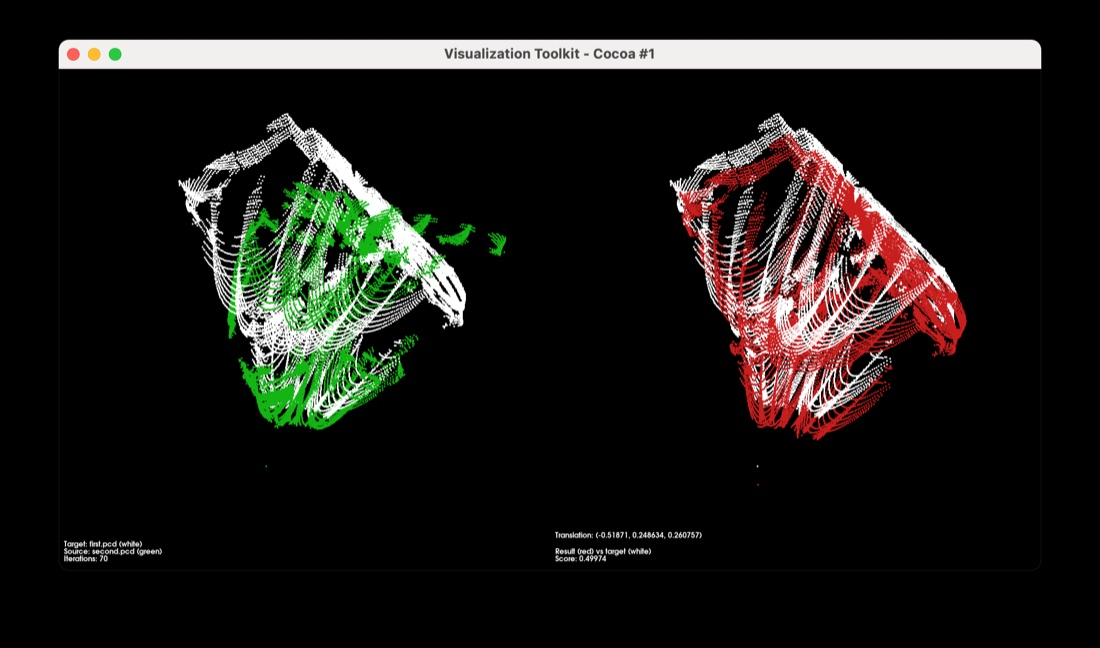
\includegraphics[width=0.78\textwidth]{figures/icp_result.jpg}
  \caption{Odometry viewer from the original deliverable. Left: first (white) and second
  (green) after levelling; right: the ICP output.}
  \label{fig:icpshot}
  \end{figure}

  % ======================================================================
  \RuleSection{Bonus --- Interactive GUI}
  \label{sec:gui}

  The viewer (\file{pclviewer.cpp}, \file{pclviewer.ui}) embeds a VTK render window in
  a Qt main window. It follows PCL's Qt tutorial and has five tabs: \emph{Setting}
  (file paths, verbose, cloud toggles), \emph{Pos} (lateral shift), \emph{SOR},
  \emph{ConeRec} (cut bottom/top, fitness) and \emph{Line} (left/right distance).
  \emph{Load} reads and levels the cloud; \emph{Compute}, or releasing any slider,
  reruns levels 1--4 and replaces the four displayed clouds (original green, cones red,
  obstacles cyan, racing line yellow).

  \begin{table}[H]
  \small
  \centering
  \renewcommand{\arraystretch}{1.05}
  \begin{tabular}{@{}llrll@{}}
  \toprule
  \textbf{Slider} & \textbf{Parameter} & \textbf{Scale} & \textbf{Range} & \textbf{Default} \\
  \midrule
  SOR       & $\alpha$ (std.\ multiplier)  & /100   & 0.5 -- 2.0      & 1.1 \\
  Cut bottom & pass-through lower $y$       & /10    & $-15$ -- $-5$ m  & $-10$ m \\
  Cut top    & pass-through upper $y$       & /10    & $-10$ -- 1.2 m   & $-0.2$ m \\
  Lateral    & shift along $z$              & /10    & $-1$ -- 1 m      & 0 m \\
  Distance   & left/right $d_{\max}$        & /10    & 0.1 -- 8 m       & 6 m \\
  Fitness    & ICP fitness threshold        & /10000 & 0.0001 -- 0.9    & 0.005 \\
  \bottomrule
  \end{tabular}
  \caption{GUI parameters. \code{QSlider} holds integers, so each value is a scaled integer.}
  \label{tab:sliders}
  \end{table}

  \paragraph{Design choices to defend.} Recomputation is triggered on
  \code{sliderReleased}, not \code{valueChanged}: a full recompute takes about 0.5 s
  (Section~\ref{sec:stats}), so recomputing on every slider tick would freeze the UI.
  ``Real-time'' in the task means that results refresh as soon as a parameter is
  set. The pipeline runs on the GUI thread; moving it to a worker
  (\code{QtConcurrent::run} plus a \code{QFutureWatcher}) would keep the window
  responsive. The project already links Qt \code{Concurrent}.

  \begin{figure}[H]
  \centering
  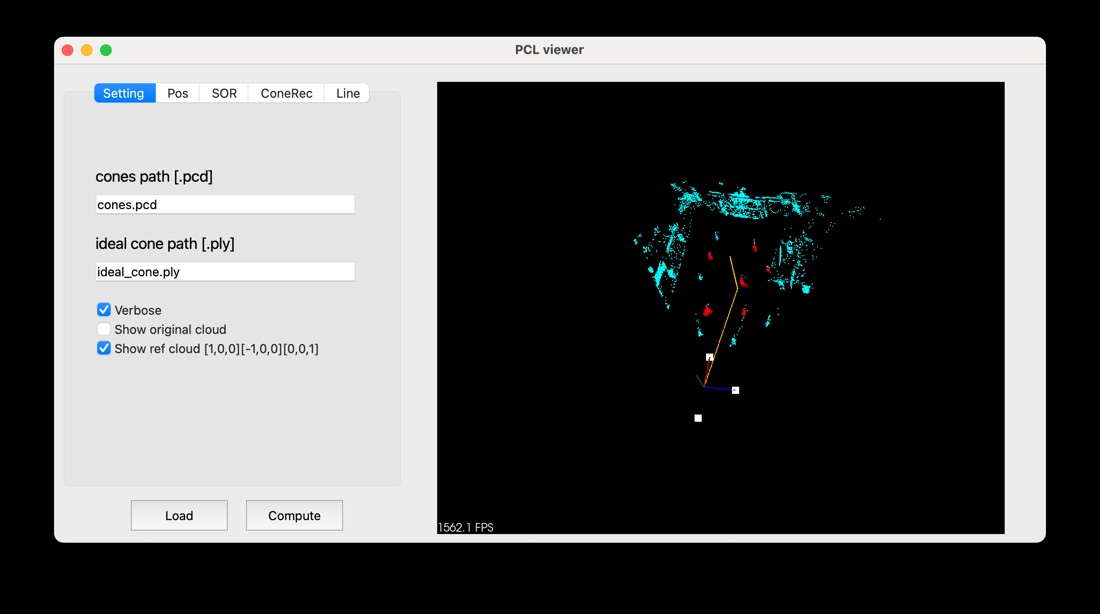
\includegraphics[width=0.55\textwidth]{figures/gui_result.jpg}
  \caption{GUI after \emph{Compute}: cones (red), obstacles (cyan), racing line
  (yellow) and the white reference points at $(\pm1,0,0)$ and $(0,0,1)$.}
  \label{fig:gui}
  \end{figure}

  % ======================================================================
  \RuleSection{C++: difficult patterns, explained}
  \label{sec:cpp}

  This section collects the parts of the code where the language does something
  non-obvious. References: \citet{stroustrup2013cpp,meyers2014effective}; Eigen:
  \citet{eigenweb}.

  \subsection{Shared pointers, aliasing and \texorpdfstring{``const''}{const} that is not const}

  \begin{lstlisting}
  // PCL: PointCloud<T>::Ptr is std::shared_ptr<PointCloud<T>>
  std::vector<int> detectCones(const pcl::PointCloud<pcl::PointXYZ>::Ptr &cloud, ...,
                               const pcl::PointCloud<pcl::PointXYZ>::Ptr &cone_model, ...)
  {
      ...
      pcl::transformPointCloud(*cone_model, *cone_model, T_center_model); // modifies the model!
  \end{lstlisting}
  \code{const Ptr\&} means the \emph{pointer} cannot be reseated. The pointee is still
  mutable: \code{const std::shared\_ptr<T>} is not \code{std::shared\_ptr<const T>}.
  \code{detectCones} therefore re-centres the caller's model in place. This is
  idempotent here (the second centring is a no-op), but it is a hidden side effect.
  PCL offers \code{PointCloud<T>::ConstPtr} for read-only inputs. Passing
  \code{shared\_ptr} by const reference avoids the atomic reference-count increment of
  a copy.

  \code{get\_cones\_cloud(src, cones\_cloud, ...)} fills its output parameter
  \emph{and} returns the same pointer inside the result struct, so in the GUI
  \code{new\_cone\_cloud} and \code{cone\_cloud} are two names for one object.

  \subsection{In-place filtering is safe in PCL}

  \begin{lstlisting}
  pass.setInputCloud(work_cloud);
  pass.filter(*work_cloud);            // input and output are the same object
  \end{lstlisting}
  This looks like it reads and writes the same buffer, but
  \code{pcl::Filter::filter} detects it (\code{if (input\_.get() == \&output)}),
  filters into a temporary and then swaps. Without that check, the code would be
  undefined behaviour.

  \subsection{Keep-organised extraction: NaN as a tombstone}

  \begin{lstlisting}
  for (const auto &cluster : clusters) {
      pcl::PointIndices::Ptr cluster_ptr(new pcl::PointIndices(cluster));
      reg_grow_extract.setIndices(cluster_ptr);
      reg_grow_extract.setNegative(true);     // keep everything EXCEPT these indices
      reg_grow_extract.setKeepOrganized(true);// ...by writing NaN, not by erasing
      reg_grow_extract.filter(*dst_cloud);
  }
  \end{lstlisting}
  All region indices were computed on the original cloud. Erasing the first region
  would shift every later index, so the second removal would delete the wrong points.
  Overwriting with NaN (a ``tombstone'') keeps every index valid. The price: later code
  must tolerate NaNs (\code{removeNaNFromPointCloud} produces an index list; the
  kd-tree skips non-finite points).

  \subsection{Structured bindings and aggregate returns (C++17)}

  \begin{lstlisting}
  struct ConeDetectionResults {
      pcl::PointCloud<pcl::PointXYZ>::Ptr centers_of_mass;
      pcl::PointCloud<pcl::PointXYZ>::Ptr cone_cloud;
  };
  auto [centers_of_mass, new_cone_cloud] = get_cones_cloud(working_cloud, cone_cloud, ...);
  auto [src_left, src_right] = cones::distinguishLeftRight(centers_of_mass, 0, 0, -45, +45, 6);
  \end{lstlisting}
  The compiler creates one hidden object of the returned type, and the two names
  refer to its members in declaration order. Returning a small struct of
  \code{shared\_ptr}s is cheap: copy elision is guaranteed for prvalues since C++17.

  \subsection{Argsort with \texttt{iota} + \texttt{sort} + a capturing lambda}

  \begin{lstlisting}
  std::vector<int> idx(N);
  std::iota(idx.begin(), idx.end(), 0);                 // 0,1,...,N-1
  std::sort(idx.begin(), idx.end(), [&](int a, int b) { // sort indices by distance
      const auto &pa = cones->points[a]; const auto &pb = cones->points[b];
      double da = (pa.x-robot_x)*(pa.x-robot_x) + (pa.y-robot_y)*(pa.y-robot_y);
      double db = (pb.x-robot_x)*(pb.x-robot_x) + (pb.y-robot_y)*(pb.y-robot_y);
      return da < db;
  });
  \end{lstlisting}
  This sorts \emph{indices} and leaves the data in place (NumPy's \code{argsort}).
  Comparing squared distances avoids $N\log N$ square roots and preserves the order.
  The comparator must be a strict weak ordering (\code{<}, never \code{<=}).
  \code{std::partial\_sort} would suffice, since only the two smallest are needed.

  \subsection{\texttt{std::vector<char>} instead of \texttt{std::vector<bool>}}

  \begin{lstlisting}
  std::vector<char> remaining(N, 1);
  remaining[first_idx] = remaining[second_idx] = 0;
  \end{lstlisting}
  \code{std::vector<bool>} is a bit-packed specialisation whose \code{operator[]}
  returns a proxy object, not a \code{bool\&}. \code{auto\& r = v[i]} does not
  compile, \code{data()} does not exist, and concurrent writes to different elements
  race. \code{std::vector<char>} avoids all three.

  \subsection{Lambdas returning references need an explicit return type}

  \begin{lstlisting}
  auto get_point = [&](int i) -> const pcl::PointXYZ& { return cones->points[i]; };
  \end{lstlisting}
  Without \code{-> const pcl::PointXYZ\&}, the lambda's return type is deduced by
  \code{auto} rules, which drop references, so every call would \emph{copy} the
  point. The reference is safe because \code{cones} outlives the lambda.
  \code{nearest\_to}, \code{safe\_turn} and \code{bad} are further local lambdas
  capturing by reference. Note that \code{rem\_idx} is rebuilt each round and captured
  by reference, so each call sees the current set.

  \subsection{A C callback with \texttt{void*} user data (NLopt C API)}

  \begin{lstlisting}
  static double objective_func(unsigned n, const double* x, double* grad, void* data) {
      auto* td = static_cast<TrackData*>(data);      // recover the type erased by void*
      ...
      if (grad) for (unsigned i = 0; i < n; ++i) grad[i] = 0.0; // LN_ algorithms pass nullptr
      return cost;
  }
  nlopt_opt opt = nlopt_create(NLOPT_LN_BOBYQA, N);
  nlopt_set_min_objective(opt, objective_func, &td); // &td travels as void*
  ...
  nlopt_destroy(opt);                                 // must be called on EVERY return path
  \end{lstlisting}
  A C library cannot call a capturing lambda or a member function, so the problem data
  travel as \code{void*}, and \code{static\_cast} restores the type. \code{static}
  gives the function internal linkage (not visible to other translation units). The
  manual \code{nlopt\_destroy} is the C way of freeing resources. The RAII version
  cannot leak on an early return:
  \begin{lstlisting}
  std::unique_ptr<nlopt_opt_s, decltype(&nlopt_destroy)> opt(
      nlopt_create(NLOPT_LN_BOBYQA, N), &nlopt_destroy);
  // or the C++ wrapper: nlopt::opt opt(nlopt::LN_BOBYQA, N);
  \end{lstlisting}
  Also worth noting: \code{objective\_func} allocates a \code{vector<vector<double>>}
  on every evaluation. A flat \code{std::vector<double>} of size $2N$, or
  \code{Eigen::Matrix2Xd}, would avoid $N$ heap allocations per call.

  \subsection{A function template with a dependent type}

  \begin{lstlisting}
  template <typename T>
  std::vector<T> linspace(T a, T b, size_t N) {
      T h = (b - a) / static_cast<T>(N-1);
      std::vector<T> xs(N);
      typename std::vector<T>::iterator x;   // 'typename': dependent name is a type
      T val;
      for (x = xs.begin(), val = a; x != xs.end(); ++x, val += h)  // comma operator
          *x = val;
      return xs;
  }
  \end{lstlisting}
  \code{std::vector<T>::iterator} depends on \code{T}, so the compiler must be told that
  it is a type (\code{typename}). \code{T} is deduced as \code{float} from the call
  site. Accumulating \code{val += h} adds rounding error; \code{a + i*h} does not.
  $N=1$ divides by zero.

  \subsection{Eigen: \texttt{rotate} post-multiplies}

  \begin{lstlisting}
  Eigen::Affine3f T = Eigen::Affine3f::Identity();
  T.translation() << 0.0, 0.0, 0.1;                          // T = Trans
  T.rotate(Eigen::AngleAxisf(M_PI/2, Eigen::Vector3f::UnitX())); // T = Trans * Rx
  T.rotate(Eigen::AngleAxisf(-M_PI, Eigen::Vector3f::UnitY()));  // T = Trans * Rx * Ry
  Eigen::Matrix3f R = transform.block<3,3>(0,0);              // fixed-size block view
  Eigen::Matrix4d M = icp.getFinalTransformation().cast<double>();
  \end{lstlisting}
  \code{rotate(R)} computes $T\leftarrow T R$ (rotation applied \emph{first} to the
  point); \code{prerotate(R)} computes $T\leftarrow RT$. Because the translation was
  set first and the rotations post-multiply, the translation is expressed in the
  \emph{output} frame. That is why the 0.1 m ends up on $z'$, the lateral axis.
  \code{block<3,3>(0,0)} is a compile-time-sized view with no copy until it is
  assigned. \code{compute3DCentroid} returns an \code{Eigen::Vector4f}, a homogeneous
  vector with $w=1$.

  \subsection{Default arguments and duplicate definitions across files}

  \code{detectCones} has default arguments in both \file{cones\_recog.h} and
  \file{cones\_recog.cpp}. This compiles only because the \file{.cpp} does not include
  its own header. If it did, the compiler would report ``redefinition of default
  argument''. Defaults belong in the declaration (header) only. The values actually
  used are those passed by \code{get\_cones\_cloud} ($-0.7$, 0.2, 0.5, 13$^\circ$),
  not the header defaults ($-0.01$, 0.3, 0.5, 20$^\circ$). Similarly,
  \code{struct cones::Result} is defined both in the header and in the \file{.cpp}.
  The One Definition Rule allows identical class definitions in different translation
  units, but if the two ever diverge, the behaviour is undefined, with no diagnostic
  required.

  \subsection{Templates and precompiled instantiations: why Debug \texorpdfstring{$\approx$}{~} Release}

  \code{pcl::IterativeClosestPoint<pcl::PointXYZ, pcl::PointXYZ>} is a class template.
  PCL ships \emph{precompiled instantiations} for common point types in
  \code{libpcl\_registration}, built in Release by Homebrew. The project's own Debug
  flags therefore barely affect the heavy work. Measured: Debug $2{,}278$ ms vs.\
  Release $2{,}260$ ms per ICP (0.8\,\%; Section~\ref{sec:stats}).

  \subsection{Qt: signals, slots, moc and the generated UI}

  \begin{lstlisting}
  class PCLViewer : public QMainWindow {
      Q_OBJECT                        // moc generates the meta-object code (CMAKE_AUTOMOC)
  public Q_SLOTS:
      void slidersReleased();
  private:
      Ui::PCLViewer *ui;              // class generated by uic from pclviewer.ui (CMAKE_AUTOUIC)
  };
  connect(ui->horizontalSlider_sor, SIGNAL(sliderReleased()), this, SLOT(slidersReleased()));
  // compile-time checked alternative:
  connect(ui->horizontalSlider_sor, &QSlider::sliderReleased, this, &PCLViewer::slidersReleased);
  \end{lstlisting}
  The string-based \code{SIGNAL}/\code{SLOT} macros are resolved at \emph{run} time:
  a typo prints a warning and the connection silently fails. The pointer-to-member
  form is checked by the compiler. \code{Ui::PCLViewer} is forward-declared and held by
  pointer, which keeps the generated header out of \file{pclviewer.h} (a compile
  firewall). It is deleted in the destructor; a \code{std::unique\_ptr} would do this
  automatically.

  \subsection{Small traps that are easy to miss}

  \begin{itemize}\sloppy
    \item \code{static\_cast<int>(initial\_sor\_std\_dev\_thr) * 100 + 100}: the cast
      binds to the variable first, so $1.1\to1$ and the result is 200, not 210.
    \item \code{pcl::console::TicToc time} is passed \emph{by value} into
      \code{processClusterForConeDetection}, so each call copies the timer.
    \item \code{\#if VTK\_MAJOR\_VERSION > 8} chooses the render-window API at compile
      time: VTK 9 needs a \code{vtkGenericOpenGLRenderWindow} attached with
      \code{setRenderWindow}, VTK 8 uses the older calls.
    \item In CMake, \code{find\_package(Qt6 QUIET ...)} falls back to Qt5 and stores
      the choice in \code{QTX}, which is used later as \code{\$\{QTX\}::Widgets}. NLopt is
      found via \code{pkg\_check\_modules}.
    \item \code{std::getenv("PERCEPTION\_HEADLESS")} enables the headless benchmark. It is
      checked \emph{after} the \code{PCLVisualizer} is constructed, so headless runs still
      pay for creating the viewer.
    \item A log message for over-tall clusters prints ``\code{<} min\_cone\_height''
      instead of ``\code{>} max\_cone\_height'' (copy-paste).
  \end{itemize}

  % ======================================================================
  \RuleSection{Statistics: what each number means and how it was obtained}
  \label{sec:stats}

  \subsection{Engineering footprint (from \texttt{STATS.md})}

  \begin{table}[H]
  \small
  \centering
  \renewcommand{\arraystretch}{1.1}
  \begin{tabularx}{\textwidth}{@{}L{3.6cm} L{1.6cm} L{4.6cm} X@{}}
  \toprule
  \textbf{Statistic} & \textbf{Value} & \textbf{How it is computed} & \textbf{Justification / caveat} \\
  \midrule
  Commits & 89 (now 90) & \code{git rev-list --count HEAD} & 89 at the snapshot; the ``stats'' commit itself is the 90th. 85 commits fall in the two-week window (28 Oct -- 12 Nov 2025), 4 on 17 Nov 2025. \\[.1cm]
  C++ files / headers & 47 / 25 & \code{git ls-files} filtered by extension & Whole repository, including R\&D prototypes and branch copies in \file{other/}, not only delivered code. \\[.1cm]
  GUI C++/header LOC & 1,862 & \code{wc -l} over the 14 files & Physical lines. 1,490 are non-blank, and about 115 are a commented-out test \code{main} in \file{racingline\_nlopt.cpp}. \\[.1cm]
  Odometry LOC & 225 & \code{wc -l main.cpp} & Before the stats commit; that commit added the 6-line headless switch, giving 231 today. \\[.1cm]
  Delivered modules & 7 & count & cone recognition, cone cloud, obstacles, left/right, racing line, viewer, odometry. \\[.1cm]
  Qt UI files & 2 & \code{*.ui} & \file{pclviewer.ui} (used) and \file{oldpclviewer.ui} (legacy). \\[.1cm]
  PCD / PLY assets & 14 / 7 & \code{git ls-files} & Includes duplicates across branches; there are 3 distinct task scans. \\
  \bottomrule
  \end{tabularx}
  \caption{Repository statistics, re-checked on 2026-10-07.}
  \label{tab:repostats}
  \end{table}

  \subsection{Runtime statistics (odometry)}

  \textbf{Method.} The odometry binary was run 10 times with
  \code{PERCEPTION\_HEADLESS=1} under \code{/usr/bin/time -l}. ICP time comes from PCL's
  \code{TicToc}, which wraps \emph{only} \code{icp.align()}. Wall, user and system time
  and peak resident set size (RSS) come from \code{time}. The run was repeated on
  2026-10-07 in both build types to check reproducibility.

  \begin{table}[H]
  \small
  \centering
  \renewcommand{\arraystretch}{1.05}
  \begin{tabular}{@{}lrrr@{}}
  \toprule
  & \textbf{STATS.md (Debug)} & \textbf{Reproduced (Debug)} & \textbf{Reproduced (Release)} \\
  \midrule
  ICP time, mean [ms]        & 2,291.18 & 2,278.47 & 2,259.64 \\
  ICP time, median [ms]      & 2,268.88 & 2,256.33 & 2,257.45 \\
  ICP time, min -- max [ms]  & 2,253.55 -- 2,401.99 & 2,208.04 -- 2,424.61 & 2,185.85 -- 2,346.50 \\
  standard deviation [ms]    & --- & 73.7 & 45.5 \\
  Frequency $1000/\bar t$ [Hz] & 0.436 & 0.439 & 0.443 \\
  CPU $=(\text{user}+\text{sys})/\text{wall}$ & 94.9\,\% & 94.6\,\% & 95.4\,\% \\
  \quad user + sys / wall [s] & $30.49+0.72$ / 32.88 & $30.64+0.61$ / 33.04 & $30.26+0.59$ / 32.35 \\
  Peak RSS                   & 115,982,336 B $=$ 110.6 MiB & 112.7 MiB & 111.1 MiB \\
  Wall time per run [s]      & 3.29 & 3.30 & 3.24 \\
  \bottomrule
  \end{tabular}
  \caption{Odometry benchmark: original figures and reproduction (10 runs each, same machine).}
  \label{tab:bench}
  \end{table}

  \paragraph{How to read each number.}
  \begin{itemize}
    \item \textbf{2,291 ms is ICP time per scan pair}, not per cloud and not the whole
      program. The other $\approx$1.0 s of each 3.3 s run is process start-up (loading
      the PCL/VTK shared libraries), reading two PCD files, two SOR passes and creating
      the viewer.
    \item \textbf{0.436 Hz} $=1000/2291.18$. It is a throughput for this pair, not a
      sensor rate. A 10 Hz LiDAR leaves 100 ms per frame, so this ICP is about
      23$\times$ too slow for real time.
    \item \textbf{94.9\,\% CPU} is $(\text{user}+\text{sys})/\text{wall}$ in the
      \code{time} convention, where 100\,\% means \emph{one fully busy core}. PCL was built
      without OpenMP (it warns at start-up), so the work is single-threaded: about 1/8
      of the machine. The remaining 5\,\% is time blocked on I/O and library loading.
    \item \textbf{110.6 MiB} $=115{,}982{,}336/2^{20}$ is the peak RSS. Two clouds of
      24,000 \code{PointXYZ} take only 2 $\times$ 24,000 $\times$ 16 B $\approx$ 0.73 MiB (PCL
      pads \code{PointXYZ} to 16 B for SIMD). Almost all of the footprint is shared
      libraries (PCL, VTK, FLANN) and the viewer.
    \item \textbf{Debug $\approx$ Release} (0.8\,\% apart) because the hot loop is in PCL's
      precompiled, optimised library code (Section~\ref{sec:cpp}).
    \item The run-to-run spread (SD 74 ms, about 3\,\%) is OS scheduling and thermal
      noise. The difference between 2,291 and 2,278 ms is within it.
  \end{itemize}

  \subsection{Runtime statistics (cone pipeline)}

  \begin{table}[H]
  \small
  \centering
  \renewcommand{\arraystretch}{1.05}
  \begin{tabular}{@{}lrl@{}}
  \toprule
  \textbf{Stage} & \textbf{Time [ms], mean $\pm$ SD} & \textbf{Complexity} \\
  \midrule
  Pass-through ($y$ band)            & 0.1          & $O(n)$ \\
  SOR ($k=50$)                      & $22.1\pm1.1$  & $O(nk\log n)$ \\
  Normal estimation ($k=50$)        & $20.1\pm0.5$  & $O(nk\log n)$ + $3\times3$ eigen-solve per point \\
  Region growing ($K=300$)          & $180.3\pm20.5$ & $O(nK\log n)$ \\
  Euclidean clustering ($r=5$ cm)    & $6.4\pm2.0$   & $O(n\log n)$ \\
  Gates + 9 ICP fits to the model   & $\approx2$    & $O(I\,m\log M)$ per cluster, $m\le500$, $M=150$ \\
  \quad \code{get\_cones\_cloud} total & $226.0\pm7.2$ & \\
  Left/right split                  & $<0.2$       & $O(N^2)$ \\
  Racing line (BOBYQA, 78 evaluations) & $\approx0.1$ & one $O(N)$ evaluation per iteration \\
  Obstacle extraction               & $266.6\pm20.8$ & dominated by its own region growing \\
  \textbf{Total}                    & $\bm{492.9\pm28.0}$ & $\Rightarrow\approx2.0$ Hz \\
  \bottomrule
  \end{tabular}
  \caption{Cone pipeline timing, 10 headless runs with GUI defaults, Release build
  (measured). Stage rows are from an instrumented replica of the same calls.}
  \label{tab:conetime}
  \end{table}

  Region growing appears twice (walls for cones, walls for obstacles) and accounts for
  about 75\,\% of the total. The obvious optimisations: compute normals and regions
  once and share them; reduce $K=300$; downsample with a voxel grid before normal
  estimation; or replace wall removal by ground-plane RANSAC plus a height band.

  % ======================================================================
  \RuleSection{Limitations and what to do next}
  \label{sec:limits}

  \begin{enumerate}
    \item \textbf{Left/right uses one coordinate} (Section~\ref{sec:l4a}). Fix the frame
      mapping, then replace the greedy split by Delaunay-based path search or
      intensity-based cone colour.
    \item \textbf{The curvature proxy is blind to reversals} (Section~\ref{sec:l4b}).
      Use the turning angle or Menger curvature; order the gates; draw all $N$
      optimised points.
    \item \textbf{Odometry is ill-conditioned and unbounded} (Section~\ref{sec:l5}).
      Bound correspondences, level the scans automatically with RANSAC, use
      point-to-plane ICP or GICP with a motion prior, and report the convergence state and
      inlier ratio instead of only ``converged''.
    \item \textbf{Thresholds tuned on one scene.} The yaw margin is 0.5$^\circ$, and the
      fitness gate is inactive on this scene. Validating on more scans, with labelled
      cones and precision/recall, is the obvious next step.
    \item \textbf{Not real-time.} 0.49 s for cones and 2.3 s for ICP, against a 0.1 s budget.
      Share normals, downsample, parallelise (OpenMP or TBB), and cache kd-trees.
    \item \textbf{Code structure.} The report itself names organisation, readability and
      memory management as the weakest areas: free functions instead of classes,
      exported magic numbers, manual resource handling.
    \item \textbf{Far-range distortion.} The report observes that cone spacing seems
      distorted at range. With $n\propto r^{-2}$, far cones have few points, so their
      centroids are noisier and biased towards the sensor. A covariance per cone would make
      this uncertainty explicit.
  \end{enumerate}

  % ======================================================================
  \RuleSection{Question-and-answer drill}
  \label{sec:qa}

  \begin{askbox}[Why LiDAR and not the camera path?]
  \small LiDAR gives metric 3D directly: no monocular scale ambiguity, no lighting
  dependence, and cone geometry can be verified with a 3D model. The camera path would
  use ORB features~\citep{rublee2011orb}, a brute-force matcher, the essential matrix
  $E=K^\top FK$ from the given intrinsics $K$ (five-point RANSAC~\citep{nister2004efficient,fischler1981ransac}),
  and pose recovery up to an unknown scale~\citep{hartley2004multiple}. LiDAR odometry
  gives translation in metres.
  \end{askbox}

  \begin{askbox}[Why region growing instead of RANSAC to remove walls?]
  \small RANSAC removes one plane per run and needs to know how many planes to remove.
  Region growing with a 1$^\circ$ normal tolerance and a 500-point minimum removes all
  large planar regions at once. Cones cannot reach 500 points (the largest has 113),
  so they are safe by construction.
  \end{askbox}

  \begin{askbox}[Why Euclidean clustering and not K-means or DBSCAN?]
  \small K-means needs $k$ in advance and assumes compact, similar-sized clusters.
  Euclidean clustering is DBSCAN with minPts $=1$: no $k$, arbitrary shapes, and noise
  handled by the size limits [8, 500]. With a 5 cm radius at 3--5 m range it separates
  cones that are about 1 m apart.
  \end{askbox}

  \begin{askbox}[What does a fitness of 0.005 mean physically?]
  \small It is a mean \emph{squared} distance in m$^2$, so the RMS residual is
  $\sqrt{0.005}=7.1$ cm. Accepted cones achieved 2.0--3.3 cm RMS. On this scene every
  candidate passed the fitness test; the yaw gate made the difference.
  \end{askbox}

  \begin{askbox}[A cone is symmetric about its axis --- why test yaw?]
  \small Yaw is a null direction of the cost for a true cone, so a local optimiser
  started at identity barely moves along it: accepted 1.2--12.5$^\circ$. Wall
  fragments must be rotated to fit the model: rejected 17.5--45.3$^\circ$. It is an
  empirical separator; 13$^\circ$ sits in the gap, and 15$^\circ$ would maximise the
  margin. A tilt check would be more principled.
  \end{askbox}

  \begin{askbox}[How do you know the 6 detections are correct?]
  \small There are no labels. The evidence: the cluster heights (0.31--0.32 m for the best
  views) match the regulation cone; the residuals are 2--3 cm; the points follow
  $n\propto r^{-1.96}$ as predicted for fixed-size objects; and the six positions form a
  plausible bend that agrees with the MATLAB prototype's input. For a real evaluation I
  would label several scans and report precision and recall per range bin.
  \end{askbox}

  \begin{askbox}[Explain the racing-line objective and the solver.]
  \small Offsets $d_i$ along the normals of the centreline, bounded by the half-widths
  so that the line stays on track; cost $=\sum\kappa_i^2+0.1\sum(\Delta d)^2$; curvature
  from finite differences (the $h$ cancels; $\varepsilon=10^{-6}$ guards against
  coincident points). BOBYQA is used because it is derivative-free and handles bounds
  natively, and $N$ is tiny: 78 evaluations, 0.1 ms. On the toy track it beat
  CasADi/IPOPT (0.05223 vs.\ 0.05305).
  \end{askbox}

  \begin{askbox}[Is the racing line on the real scene correct?]
  \small No, and I can explain why: the split orders the cones so that the centreline
  folds back, and the $\sin\theta$ proxy assigns zero cost to a 180$^\circ$ reversal,
  so the optimiser returns a folded line with $J\approx0$. Fixes: correct the
  left/right frame bug, order the gates along the track, and use the signed turning angle
  or Menger curvature. The optimisation machinery itself is validated on the toy track.
  \end{askbox}

  \begin{askbox}[Is the odometry result reliable?]
  \small It is reproducible (identical numbers across runs and machines), and the
  conversion to a displacement is correct: $-R^\top\bm t$, about 0.54 m forward and 0.23 m
  lateral. But ICP hit its 70-iteration cap with unbounded correspondences, close inliers
  fell from 12.7\,\% to 4.1\,\%, and GICP and bounded ICP give very different answers.
  So the pair is ill-conditioned. I would bound correspondences, level automatically,
  use GICP or point-to-plane ICP with a motion prior, and check the Hessian
  conditioning.
  \end{askbox}

  \begin{askbox}[Is it real-time? Where would you optimise?]
  \small No: 0.49 s for cones (2 Hz) and 2.3 s for ICP (0.44 Hz), against 100 ms at
  10 Hz. Region growing is about 75\,\% of the cone time and runs twice, so share it,
  downsample, and lower $K$. For ICP: voxel-downsample to a few thousand points, bound
  correspondences (fewer iterations), use OpenMP (PCL was built without it), or switch
  to a tuned point-to-point pipeline such as KISS-ICP~\citep{vizzo2023kiss}.
  \end{askbox}

  \begin{askbox}[Why is a Debug build as fast as Release?]
  \small The time is spent inside PCL's precompiled template instantiations
  (\code{IterativeClosestPoint<PointXYZ,PointXYZ>}, FLANN kd-tree), which are always
  optimised. Our own code is a thin layer. Measured difference: 0.8\,\%.
  \end{askbox}

  \begin{askbox}[Point-to-point vs.\ point-to-plane ICP?]
  \small Point-to-point minimises Euclidean distances between matched points and has
  an exact SVD solution per iteration. Point-to-plane minimises the distance along the
  target normal, so points may slide along surfaces. It converges in fewer iterations on
  man-made scenes but needs normals and a linearised solve~\citep{chen1992object,rusinkiewicz2001efficient}.
  \end{askbox}

  \begin{askbox}[What would you change first with one more week?]
  \small (1) Fix the left/right frame and use Delaunay midpoints; (2) make the
  curvature reversal-aware; (3) bounded, robust, levelled registration with an
  $SE(2)$ constraint; (4) wrap the pipeline in classes with a parameter struct shared by
  the GUI and the CLI, plus unit tests per stage; (5) run the computation on a worker
  thread.
  \end{askbox}

  % ======================================================================
  \RuleSection{Formula sheet}
  \label{sec:formulas}

  \begin{table}[H]
  \small
  \centering
  \renewcommand{\arraystretch}{1.35}
  \begin{tabularx}{\textwidth}{@{}L{3.6cm} X@{}}
  \toprule
  Inverse transform & $T^{-1}=\begin{bmatrix}R^\top&-R^\top\bm t\\\bm 0^\top&1\end{bmatrix}$ \\
  Rotation angle / axis & $\theta=\arccos\frac{\tr R-1}{2}$,\quad $\bm u=\frac{1}{2\sin\theta}(r_{32}-r_{23},\,r_{13}-r_{31},\,r_{21}-r_{12})$ \\
  SOR & keep $\bar d_i\le\mu+\alpha\sigma$, \quad $\bar d_i=\frac1k\sum_{j\in\mathcal N_k(i)}\norm{\bm p_i-\bm p_j}$ \\
  Normal, curvature & $\bm n=\bm v_0(C)$, \quad $\sigma=\lambda_0/(\lambda_0+\lambda_1+\lambda_2)\in[0,\tfrac13]$ \\
  Region growing & join if $\lvert\bm n_s\cdot\bm n_q\rvert\ge\cos\theta_{\text{th}}$; seed if $\sigma<c_{\text{th}}$ \\
  ICP step & $H=\sum(\bm p_i-\bar{\bm p})(\bm q_i-\bar{\bm q})^\top=U\Sigma V^\top$, \ $R=V\,\mathrm{diag}(1,1,\det VU^\top)U^\top$, \ $\bm t=\bar{\bm q}-R\bar{\bm p}$ \\
  Fitness & $F=\frac1n\sum\min_j\norm{T\bm p_i-\bm q_j}^2$ [m$^2$], \ RMS $=\sqrt F$ \\
  Yaw (about $y$) & $\psi=\atantwo(r_{13},r_{33})$ \\
  Turning angle & $\delta=\wrap\big(\atantwo(\bm b)-\atantwo(\bm a)\big)$, or $\atantwo(\bm a\times\bm b,\ \bm a\cdot\bm b)$ \\
  Discrete curvature & $\kappa=\dfrac{\bm a\times\bm b}{(\norm{\bm a}^2+\varepsilon)^{3/2}}$; \ Menger $=\dfrac{2\sin\theta}{\norm{\bm p_{i+1}-\bm p_{i-1}}}$ \\
  Racing line & $\min_{\lvert d_i\rvert\le w_i}\ \sum\kappa_i^2+\lambda\sum(d_{i+1}-d_i)^2$, \ $\bm p_i=\bm m_i+d_i\bm n_i$ \\
  Odometry & $\bm p^{(2)}=T\bm p^{(1)}$ $\Rightarrow$ displacement $=-R^\top\bm t$ \\
  Density & $n\propto r^{-2}$ (fitted exponent $-1.96$) \\
  Throughput, CPU & $f=1000/\bar t_{\text{ms}}$ Hz; \ CPU $=(\text{user}+\text{sys})/\text{wall}$ (100\,\% = one core) \\
  \bottomrule
  \end{tabularx}
  \caption{Formulas to have at your fingertips.}
  \label{tab:formulas}
  \end{table}

  % ======================================================================
  \bibliographystyle{abbrvnat}
  \bibliography{references}

  \end{document}
